\newif\ifPDF
\ifx\pdfoutput\undefined\PDFfalse
\else\ifnum\pdfoutput > 0\PDFtrue
	\else\PDFfalse
	\fi
\fi

\ifPDF
	\documentclass[pdftex,11pt,openany,twoside]{book}
	\RequirePackage[hyperindex,colorlinks,plainpages=false]{hyperref}
	\hypersetup{pdfauthor={Heng Li},linkcolor=blue,citecolor=blue,urlcolor=blue}
	\usepackage{graphicx}
	\DeclareGraphicsRule{*}{mps}{*}{}
\else
	\documentclass[11pt,openany,twoside]{book}
	\usepackage{graphicx}
	\newcommand{\href}[2]{\textcolor{MYBLUE}{#1}}
\fi


\usepackage[%paperwidth=18.4cm, paperheight=26cm,
body={14.6true cm,22true cm},
twosideshift=0 pt,
%headheight=1.0true cm
]{geometry}

\usepackage{caption2}
\usepackage{fancyhdr}
\pagestyle{fancy}
% with this we ensure that the chapter and section
% headings are in lowercase.
\renewcommand{\chaptermark}[1]{\markboth{\chaptername \ \thechapter. \ #1}{}}
%\renewcommand{\sectionmark}[1]{\markright{\thesection\ #1}}
\fancyhf{} % delete current setting for header and footer
\fancyhead[LE,RO]{\bfseries\thepage}
\fancyhead[LO]{\bfseries\leftmark}
\fancyhead[RE]{\bfseries Constructing TreeFam Database}
\renewcommand{\headrulewidth}{0.5pt}
\renewcommand{\footrulewidth}{0pt}
\addtolength{\headheight}{0.5pt} % make space for the rule
\addtolength{\headwidth}{10pt} % make space for the rule
\fancypagestyle{plain}{%
\fancyhead{} % get rid of headers on plain pages
\renewcommand{\headrulewidth}{0pt} % and the line
}

\sloppy

\usepackage{amsmath,amssymb,amsfonts}
\usepackage[usenames,dvips]{color}
\usepackage{makeidx}

\usepackage{flafter}
\usepackage[below]{placeins}
\usepackage{floatflt}

\definecolor{MYRED}{rgb}{1,0,0}
\definecolor{MYBLUE}{rgb}{0,0,1}
%\newcommand{\lhcomm}[1]{\textcolor{MYRED}{#1}}
\newcommand{\lhcomm}[1]{#1}

\addtolength{\headsep}{-0.1cm}
\addtolength{\footskip}{-0.1cm} 

\renewcommand{\textfraction}{0.15}
\renewcommand{\topfraction}{0.85}
\renewcommand{\bottomfraction}{0.65}
\renewcommand{\floatpagefraction}{0.60}

\renewcommand{\captionfont}{\fontsize{10pt}{12pt}\selectfont}

\addtolength{\oddsidemargin}{1.2cm}
\addtolength{\evensidemargin}{-1.2cm}

%\addtolength{\textwidth}{3cm}
%\addtolength{\hoffset}{-1.5cm}
%\addtolength{\textheight}{4cm}
%\addtolength{\voffset}{-2cm}

\makeindex


\newcommand{\lhchild}{\mathrm{chi}}
\newcommand{\lhparent}{\mathrm{par}}
\newcommand{\lhlca}{\mathrm{lca}}
\newcommand{\lhopt}{\mathrm{opt}}
\newcommand{\lhloss}{\mathrm{loss}}
\newcommand{\lhspace}{\hspace{20pt}}

\usepackage{bioinformatics}
\bibliographystyle{bioinformatics}

%\title{Constructing \lhcomm{the} TreeFam Database}
%\author{Heng Li}
%\date{14JAN2006}

\begin{document}

%\maketitle

\begin{titlepage}
\thispagestyle{empty}
\begin{center}
\begin{verbatim}
  
\end{verbatim}
\vspace{5cm}
{\bf\huge CONSTRUCTING THE TREEFAM}\\
\vspace{0.5cm}
{\bf\huge DATABASE}\\
\vspace{4cm}
{\LARGE Li Heng\\
\vspace{0.2cm}
Directed by Zheng Wei-mou \\
\vspace{0.2cm}
The Institute of Theoretical Physics,\\
Chinese Academic of Science\\
\vspace{3cm}
May, 2006}\\
\end{center}
\end{titlepage}

\setcounter{page}{1}
\addcontentsline{toc}{chapter}{Abstract}
\chapter*{Abstract}
TreeFam is a database of phylogenetic trees of gene families. It aims
to develop a curated resource that presents the accurate evolutionary
history of all animal gene families, as well as reliable orthologs and
paralog assignment.
In developing TreeFam, four novel algorithms
were designed to improve the accuracy of tree building or to serve
special needs for development. The first is \lhcomm{a} constrained neighbour-joining
that efficiently adds new sequences to an existing tree while maintaining
the original topology at the same time. This method is used to expand
a seed tree to a full tree without losing any information added by
manual curation. The second algorithm is \lhcomm{a} leaf reordering that
orders the leaves of a tree according to the weights of leaves.
\lhcomm{When it is drawn as a} picture, one tree can be displayed in different
ways, depending on the order of leaves. This algorithm helps to
display trees in a \lhcomm{consistent algorithm} and facilitates
visual examination of trees, which is particularly helpful when
comparing two trees. Thirdly, duplication and loss inference
is fit into a more general theoretical framework and extended to allow for
a multifurcated species tree. \lhcomm{A fourth algorithm has also been developed, 
which is a new algorithm for merging trees.}
\lhcomm{The tree merge algorithm} itself is not a tree building algorithm, but it
reconstructs an optimal tree from several trees
that are built from an identical sequence set with different tree building
methods. The resultant tree \lhcomm{should} combine the advantages
of, and so outperform, all the candidates. This is \lhcomm{shown to occur successfully}
in a large-scale benchmark presented in the last chapter.
This benchmark is one of the few evaluations that are based on real data
\lhcomm{in the phylogenetics literature}.
It also \lhcomm{highlights the fact} that each tree-building algorithm has its own strength,
although ML and parsimonious methods are slightly better in general.

{\flushleft {\bf Keywords:} molecular phylogenetics, tree reconstruction, database}

\addcontentsline{toc}{chapter}{Acknowledgements}
\chapter*{Acknowledgements}
First of all, I am most grateful to my supervisor, Wei-mou Zheng. It was him who
took me to the realm of bioinformatics, and it was him who gave me both strict instruction and full flexibility,
which brought me a meaningful and colorful PhD life.

Next thanks go to Jun Wang and all my friends and colleagues in Beijing Genomics Institute (BGI), Chinese Academic of Science.
I spent most of my PhD in BGI. It was them who gave me three happy yet thrilling years in my life.
I particularly thank Jun Wang for his providing me the opportunity to collaborate with the Sanger TreeFam group,
and thank Tao Liu for his assist and support over three years even when I overlooked his role at the beginning.

With the same passion I appreciate the generous help and instruction from Sanger TreeFam group including
Richard Durbin, Avril Coghlan, Jean-Karim H\'{e}rich\'{e}, Lachlan James Coin, and Alan Moses. Richard is the father
of TreeFam. He raised the whole idea about TreeFam. Without him, there would be no TreeFam, not to speak my thesis.
Avril, Jean-Karim and Alan
read through this thesis and gave me numerous useful remarks and hints on further improvement. I particularly thank them
for their patience with my poor English. Lachlan and Avril also helped to revise an earlier version of
Chapter~\ref{chap:merge}. Their insightful opinions made this chapter more solid and generalized.
In addition, I learnt a lot from the communications with Sanger group, either by e-mail or in TreeFam workshop.
TreeFam is always the result of group work.

I also wish to show my gratefulness to my Danish friends, especially to Lars Bolund who provided me
a peaceful place and harmonious evironment where I could focus on TreeFam project and my thesis in 2005.
I owe a lot to him and to all my Danish friends. At the same time I want to thank to
Professor Bai-lin Hao for his kind instructions, to Ms. Ling Guo for her help when I was
in BGI, and to all my classmates and roommates of the Institute of Theoretical Physics
(ITP) for their help in these years.

At last, a big thank you to my dear prarents and my girlfriend for their silent support all the time.

\tableofcontents
\addcontentsline{toc}{chapter}{Contents}
\listoffigures
\listoftables

\chapter{Introduction}

Phylogenetics\index{phylogenetics} is the science of studying the evolutionary
relationships (phylogenies\index{phylogenetics!phylogeny}) of a group of organisms~\cite{baldauf03} or genes. One of the fundamental
hypotheses of phylogenetics is that all organisms on Earth had a common ancestor and
can be represented as trees. This hypothesis can be dated back to the era of Darwin
and \lhcomm{is} supported by various studies on the similarity of molecular mechanisms of
organisms~\cite{durbin98}. Successfully reconstructing the tree of life has long been
the dream, and also the aim, of evolutionists.

Traditionally, phylogenetic trees are reconstructed by examining and comparing
morphological characters (both from living and fossilized organisms), which
was and still is a time-consuming and specialized endeavor~\cite{cotton03}.
Since the publication of Zuckerkandl and Pauling's original paper~\cite{zuckerkandl65} that
showed molecular sequences could also serve as characters, molecular phylogenetics
found its own position and has become
a distinct and fruitful direction of phylogenetics in recent years with
rapidly increasing sequence data. It not only
produces \lhcomm{an} overwhelming amount of information to biologists, but also
inspires the development of computer science and statistics.

\section{Background}

Whereas reconstructing the tree of life is one of the central topics of phylogenetics,
reconstructing the phylogeny of each gene family shows the strength of phylogenetic methods
to most of molecular biologists. Phylogenies of gene families not only present
the history of gene evolution, but also hold the key to gene annotations
across species. The functional annotations or experimental results of genes in one
species can be transferred to another when the history of related gene families is
clear. This integrates the efforts of gene annotation in different species and is vital
to annotations, especially to the annotations of a newly sequenced species.
Of the same importance, reconstructing of gene phylogenies is the premise of discovering
the priciples of gene evolution, which further provides clues to interpret gene functions.
For example, the difference of selective pressures on genes implies functional shifts between
them. Meaningful mutations, pseudogenes and interaction networks may also be inferred
with the help of gene phylogenies~\cite{ng03,coin04}. In addition, reconstructing phylogenies of gene families paves
the way for other related evolutionary studies, such as intron evolution and genome-wide
duplications.

Given the importance of gene phylogenies, many databases have been developed to
present the history of each gene family, including KOG~\cite{tatusov03}, PANTHER~\cite{mi05}, SYSTERS~\cite{meinel05}
PhIGs~\cite{dehal05}, Ensembl-compara~\cite{hubbard05}, OrthoMCL~\cite{li03} and HOGENOM~\cite{dufayard05}.
These efforts greatly boost the studies of gene evolution, but they are all faced with
a common problem: how can a reliable phylogenetic tree be reconstructed?
And this problem is, unfortunately, always one of the hardest topics in the area of bioinformatics~\cite{delsuc05}.
Sequences of poor data quality (such as incorrect gene annotation or few informative sites)
and unrealistic underlying evolutionary model (such as assuming that different lineages
have evolved at the same rate) may greatly affect the accuracy of tree building.
No automatic algorithm can reconstruct an accurate tree all the time. To make a phylogenetic database
practically useful, this problem has to be solved.

\section{Overview of the Thesis}

TreeFam is a (gene) tree family database. Phylogenetic trees are the central elements.
In developing TreeFam, the tree building difficulties are solved in two directions. First,
a new algorithm, tree merge, is developed to improve the quality of automatic trees, and second,
mannual curation is applied to further get higher accuracy with the help of the constrained neighbour-joining
algorithm. This thesis presents the details to these algorithms and also covers 
most of topics related to the construction of TreeFam, including
basic concepts, pipelines, additional algorithms, and implementations. In attempt to keep this
thesis as an academic one, technical issues are placed in the appendix even though these
issues might \lhcomm{have been} of the same importance as academic aspects when TreeFam database
was set up.

\begin{figure}
\begin{center}
\includegraphics[width=0.7\textwidth]{chapflow}
\caption{Relationships between chapters.}\label{fig:chapflow}
\end{center}
\end{figure}

In the following section of this chapter, \lhcomm{the} biological backgrounds and mathematical
notations will be clarified. Chapter~\ref{chap:treefam} describes the philosophy and structure of \lhcomm{the} TreeFam database.
Chapter~\ref{chap:buildtree} covers various small yet important topics on \lhcomm{the} tree-building process, particularly
two algorithms, constrained neighbour-joinining and leaf reordering algorithm, which
are inspired by \lhcomm{the} TreeFam project. Chapter~\ref{chap:dli} extends the traditional
tree-reconciliation procedure so as to allow for a multifurcated species tree
and presents discussion about tree mapping. Chapter~\ref{chap:merge} describes tree merge algorithms,
which is the chief effort in improving the quality of automatic trees.
And in Chapter~\ref{chap:benchmark}, various tree-building algorithms are evaluated, \lhcomm{using the curated
TreeFam trees as a test set}. The relationships between chapters are showed in Figure~\ref{fig:chapflow}.

Except this introductory chapter, most of the results showed in this thesis have not been published yet.
Although Chapter~\ref{chap:treefam} is based on our paper~\cite{li06}, it still differs much from
the published works. Some important results in the thesis are expected to be published in the following months.

\section{Phylogenetic Terminology}
\emph{Phylogeny}\index{phylogenetics!phylogeny} denotes the evolutionary relationships of a group of organisms or genes.
It can be represented as a tree, called a \emph{phylogenetic tree}\index{tree!phylogenetic tree}.
\emph{Phylogenetics}\index{phylogenetics} is the field of biology that studies phylogenies.
It includes the reconstruction of phylogenies and \lhcomm{the study of the factors that affect
phylogenies, and the biological meaning that phylogenies reveal}.

\begin{figure}[!hb]
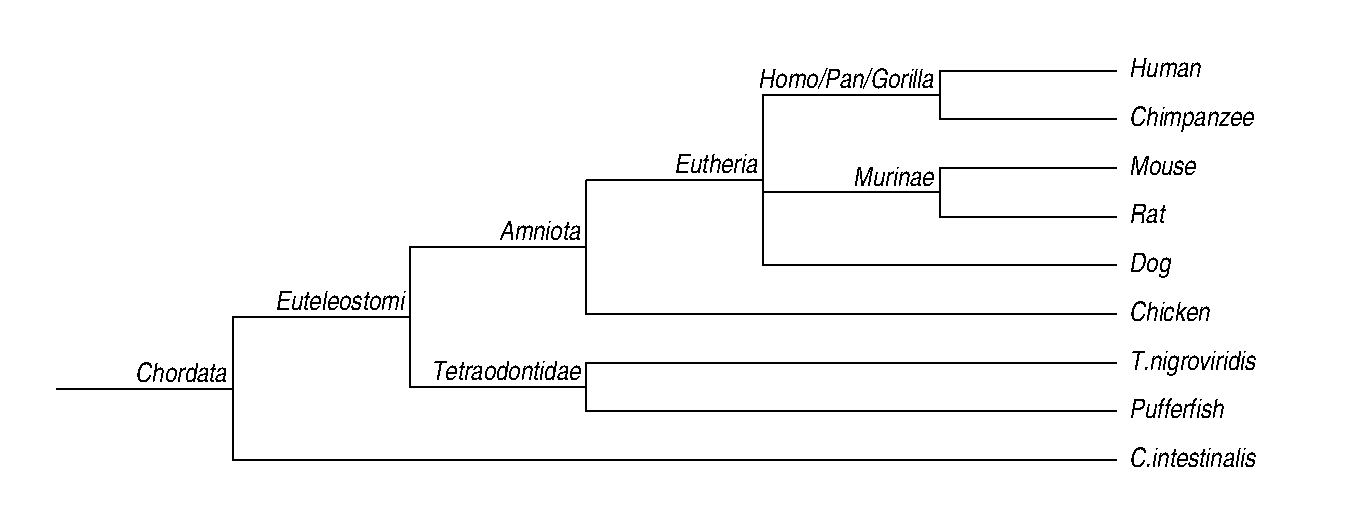
\includegraphics[width=\textwidth]{spec}
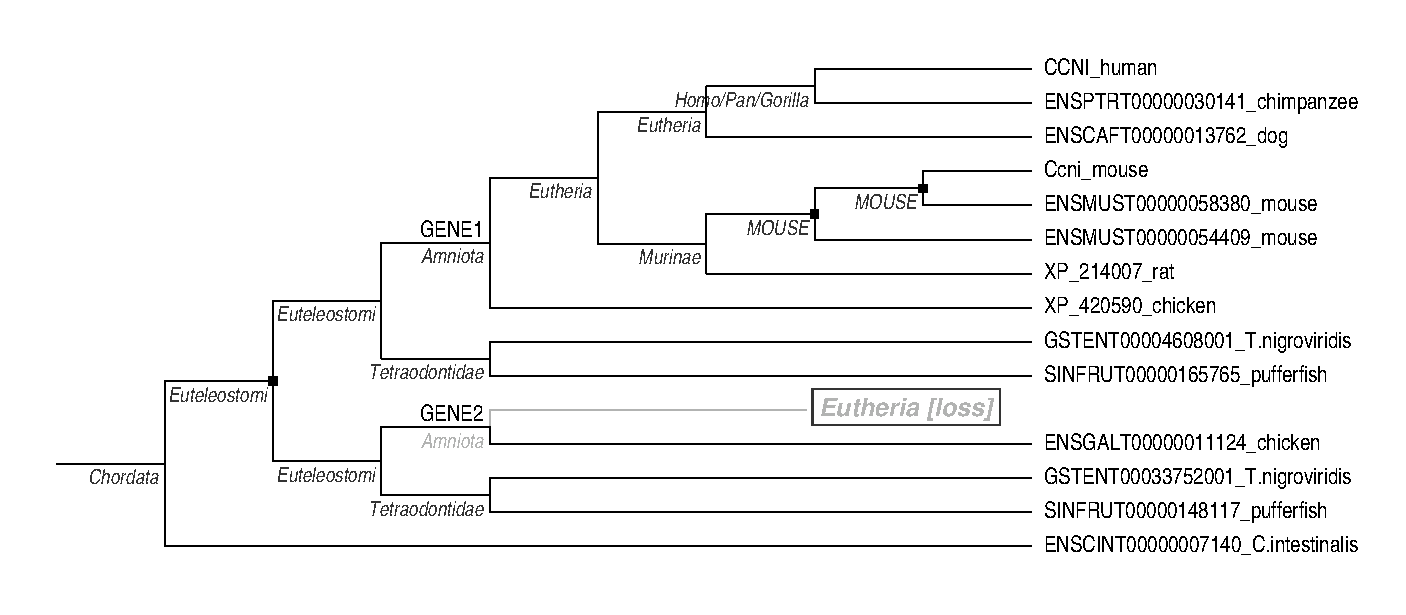
\includegraphics[width=\textwidth]{gtree}
\caption[Examples of a species tree and a gene tree]
	{Example of a species tree and a gene tree. The top figure shows a species tree of {\it Chordata} phylum.
	This tree will be used throughout this thesis.
	The bottom shows the gene tree of {\it Cyclin I} sub- gene family. A slant name beside the internal node
	shows the ancestral species that contained the correponding ancestral gene. In this gene tree,
	the human gene {\sf CCNI\_human} is 1:1 orthologous to {\sf XP\_420590\_chicken} because
	they are descendant from a single gene in {\it Amniota}, the LCA of {\it human} and {\it chicken}. But this human gene is only
	homologous to, but not orthologous to,
	{\sf ENSGALT00000011124\_chicken} because although both genes
	are descendant from a single gene in {\it Euteleostomi}, the human gene is a descendant of {\sf GENE1} in {\it Amniota}
	while {\sf ENSGALT00000011124\_chicken} of {\sf GENE2}. In addition, this gene tree also shows several 1:n orthologs.
	For example, gene {\sf ENSCINT00000007140\_C.intestinalis} is an 1:2 ortholog of {\sf SINFRUT00000165765\_pufferfish}
	and {\sf SINFRUT00000148117\_pufferfish}. The bottom figure will be reexamined in Chapter~\ref{chap:dli}
	where more details will be presented.}\label{fig:spectree}
\end{figure}

In this thesis, two types of trees will be involved: species trees and gene trees.
Strictly speaking, a \emph{species}\index{species}
is ``a group of organisms capable of interbreeding freely with each other but not with members of other
species''~\footnote{\href{http://www.edu.gov.nf.ca/curriculum/teched/resources/glos-biodiversity.html}
{http://www.edu.gov.nf.ca/curriculum/teched/resources/glos-biodiversity.html}}.
A \emph{species tree}\index{tree!species tree} (Figure~\ref{fig:spectree}) describes the evolution relationships between species.
Each of its external nodes (or terminal nodes, or leaf nodes, or leaves)
stands for a present species\index{species!present species} that can be observed nowadays, while each
internal node for an ancestral species\index{species!ancestral species} in history.
An ancestral species is usually named after \lhcomm{the taxon that represents its descendant species}.
For example, when we say species {\it Eutheria}\index{Eutheria@\textit{Eutheria}}, we mean the ancestral species from which
all species in \lhcomm{the taxon {\it Eutheria} are} descendant.
\lhcomm{The} science of naming and classifying organisms is called \emph{taxonomy}\index{taxonomy}, a branch of
phylogenetics.
Taxonomists would prefer to term a (present or ancestral) species as a \emph{taxon}\index{taxonomy!taxon}
({\it pl.} taxa\index{taxonomy!taxa})\footnote{According to taxonomy, all species are classified
at six major levels. In an order from most genernal to most specific, the six levels are
kingdom\index{kingdom}, phylum\index{phylum}, class\index{class}, order\index{order},
family\index{family}, genus\index{genus} and species. For example, {\it human} belongs to
such groups: {\it Animalia} (kingdom), {\it Chordata} (phylum), {\it Mammalia} (class),
{\it Primates} (order), {\it Hominidae} (family), {\it Homo} (genus), and {\it Homo sapiens} (species).}

A \emph{gene}\index{gene} is defined as: ``A DNA segment that contributes to phenotype/function. In
the absence of demonstrated function a gene may be characterized by sequence, transcription or
homology''~\footnote{\href{http://www.gene.ucl.ac.uk/nomenclature/guidelines.html}
{http://www.gene.ucl.ac.uk/nomenclature/guidelines.html}}.
Genes are related in the context of evolution. {\it Homologs}\index{ortholog!homolog} are genes
that are descendant from a single gene~\cite{koonin05}. {\it Orthologs}\index{ortholog} are genes in different
species that originate from a single gene in the last common ancestor of these species~\cite{remm01}; furthermore,
we say $m$ genes in one species and $n$ genes in another form $m:n$ orthologs if
the $m+n$ genes are all descendant from a single gene in the LCA of the two species (Figure~\ref{fig:spectree}).
By definition, orthologs must be homologs, and they are closer homologs;
homologs that are not orthologs are {\it paralogs}\index{ortholog!paralog}.
Homologous genes form a \emph{gene family}\index{gene!gene family} which
is defined a group of gene that are descendant \lhcomm{of} a single ancestral gene. The evolutionary relationships
between genes in a gene family can also be represented as a tree, named \emph{gene tree}\index{tree!gene tree}.
Similarly, each external node of a gene tree stands for a present gene\index{gene!present gene} that
can be observed nowadays, while each internal node for an ancestral gene\index{gene!ancestral gene} that
only existed in history.

Species trees and gene trees are related: species trees can be inferred from gene trees, and
gene trees reflect patterns in species trees. At the same time, gene trees can differ from
species trees due to the existence of duplications\index{duplication}, losses\index{loss}, and
\lhcomm{lateral gene transfer (LGT)}\index{LGT, Lateral Gene Transfer}, which can, in turn, be inferred by reconciling
a gene tree and a species tree. One of the exceptional features of TreeFam, and therefore
of this thesis, is to untangle the relations between species trees and gene trees.
Many meaningful conclusions, such as the functional evolution and differentiation of genes,
can be made when these relations are resolved. Such relations also help to reconstruct reliable gene trees.

% kingdom phylum (subphylum) class (subclass) order (suborder) family genus species
% Animalia Chordata Vertebrata Mammalia Eutheria Primates Catarrhini Hominidae Homo

\section{Terminology \lhcomm{for} Trees}

\subsection{Common terminology \lhcomm{for} trees}
In graph theory, a tree is a connected graph that contains no cycle.
It is comprised of \emph{nodes}\index{node} (vertices\index{vertex}) and \emph{branches}\index{branch}
(edges\index{edge@edge, {\it see also} branch})
which connect nodes. A node can be external\index{node!external node} (terminal\index{node!terminal node})
if it is only attached to one branch,
or internal\index{node!internal node} if two or more branches are joined by the node.
An external node is also termed as a \emph{leaf}\index{leaf}\index{node!leaf node}.

Strictly speaking, every true phylogenetic tree is a \emph{rooted tree}\index{tree!rooted tree} that presents the direction of
evolution. The root\index{node!root node} node is regarded as the earliest ancestor of all the species or genes
in the tree. In a rooted tree, each internal node has its children; except the root, each node has
one parent. The branches close to the root are called higher or deeper
branches\index{branch!deeper branch}\index{branch!higher branch}, while close to
the leaves called lower branches\index{branch!lower branch}.
Given a set of nodes, the lowest ancestral node from which all the given nodes are descendant
is called \emph{LCA} (Last Common Ancestor)\index{LCA, last common ancestor}. A node and
all the nodes descendant from it form a \emph{clade}\index{clade}.

A true phylogenetic tree is also a \emph{binary tree}\index{tree!binary tree} in which each internal node has exactly two children.
A binary tree is also called a \emph{resolved tree}\index{tree!resolved tree} in the sense that every evolutionary event
is presented in the tree. However, if two successive events happened in \lhcomm{a} short time,
they can be hardly discriminated when the tree is reconstructed. In practice, nodes having
three or more children are still allowed. These nodes are called
\emph{polytomies}\index{polytomy@polytomy, \textit{see also} multifurcated node}
or \emph{unresolved nodes}\index{node!unresolved nodes} or
\emph{multifurcated nodes}\index{node!multifurcated node}.
A tree containing polytomies is an \emph{unresolved tree}\index{tree!unresolved tree}
or \emph{multifurcated tree}\index{tree!multifurcated tree}.
The widely used NCBI taxonomy tree~\cite{wheeler05} is a multifurcated tree.

\subsection{Representation of trees}

The most intuitive way to view a tree is to display it as an {\bf image}. However, an image can
neither be directly described in mathematical language nor be easily parsed by a computer program.
Thus it is necessary to introduce abstract languages to shape a tree and to describe
related algorithms as well.

Three types of representations will be used in the thesis: graph representation\index{representation!graph representation},
string representation\index{representation!string representation} and
set representation\index{representation!set representation}. The first two will be explained
here and the third one will appear in Chapter~\ref{chap:merge} where set
representation, being more abstract, helps to clarify the concepts and proof
in a strict manner.

\subsubsection{Graph representation: definitions and notations}

Definitions and notations in this section will be used \lhcomm{throughout} the thesis,
except in Chapter~\ref{chap:merge} where new notations will be introduced
to facilitate specific aims. Only \emph{rooted} \lhcomm{trees} will be discussed here
as any phylogenetic tree is rooted given the assumption that all organisms
on Earth had a common ancestor. In Section~\ref{sec:root-tree}, we
will come to the topic \lhcomm{of} how to find the root of an unrooted tree.

Let $T$ be a \emph{rooted} tree and $V(T)$ be the set of nodes in $T$. \lhcomm{Let $V_E(T)$ and
$V_I(T)$ be} the set of external nodes (or leaves) and internal nodes,
respectively. Given a node $v$, its direct descendants form $\lhchild(v)\subset V(T)$,
$v$'s children set, and $v$ is a child of $\lhparent(v)\in V(T)$, the parent node
of $v$.

For $u,v\in V(T)$, we write $u<v$ or $v>u$ if $u$ is a descendant of $v$. The set
of external nodes that are \lhcomm{descendent} from $v$ is defined as:
\begin{equation}\label{equ:omega}
\omega_T(v)=\{u\in V_E(T):u\leq v\}.
\end{equation}
Similarly, the set of external nodes of set $A\subset V(T)$ form the set:
\begin{equation}
\omega_T(A)=\bigcup_{u\in A}\omega_T(u).
\end{equation}
Sometimes, we might abbreviate $\omega_T(v)$ as $\omega(v)$ if $T$ can be
understood from the context.

Next, we seek to construct a subtree of $T$.
For a node set $A$, we denote by $\lhlca(A)$ the last common ancestor (or LCA)\index{LCA, last common ancestor} of $A$,
which is the lowest node ancestral to all the nodes in $A$. Let $T|_A$ be the subtree\index{subtree}
comprising of only those paths in $T$ that connect $\omega(A)$. Thus, the node set of $T|_A$ is:
\begin{equation}
V(T|_A)=\{v\in V(T):\omega_T(v)\cap\omega_T(A)\neq\emptyset\}
\end{equation}
The root of $T|_A$ is $\lhlca(A)$. We also write $T|_{\{v\}}$ as $T|_v$ for simplicity. Figure~\ref{fig:concept}
shows an example related to these concepts.

\begin{figure}[!hb]
\begin{center}
\setlength{\unitlength}{0.7cm}
\begin{picture}(18,6)
% left
\put(0,2){\line(1,1){4}}
\put(2,2){\line(-1,1){1}}
\put(4,2){\line(0,1){4}}
\put(8,2){\line(-1,1){4}}
\put(6,2){\line(1,1){1}}
\put(-0.2,1.3){1}
\put(1.8,1.3){2}
\put(3.8,1.3){3}
\put(5.8,1.3){4}
\put(7.8,1.3){5}
\put(1.5,2.8){6}
\put(7.5,2.8){7}
\put(4.5,5.8){8}
\put(0,2){\circle{0.1}}
\put(2,2){\circle{0.1}}
\put(4,2){\circle{0.1}}
\put(6,2){\circle{0.1}}
\put(8,2){\circle{0.1}}
\put(1,3){\circle{0.1}}
\put(7,3){\circle{0.1}}
\put(4,6){\circle{0.1}}
% right
\put(14,2){\line(0,1){4}}
\put(18,2){\line(-1,1){4}}
\put(9.8,1.3){1}
\put(11.8,1.3){2}
\put(13.8,1.3){3}
\put(15.8,1.3){4}
\put(17.8,1.3){5}
\put(11.5,2.8){6}
\put(17.5,2.8){7}
\put(14.5,5.8){8}
\put(10,2){\circle*{0.1}}
\put(12,2){\circle*{0.1}}
\put(14,2){\circle{0.1}}
\put(16,2){\circle*{0.1}}
\put(18,2){\circle{0.1}}
\put(11,3){\circle*{0.1}}
\put(17,3){\circle{0.1}}
\put(14,6){\circle{0.1}}
\put(3.8,0){$T$}
\put(13.8,0){$T|_A$}
\end{picture}
\caption[Example tree used to illustrate basic concepts]{Example tree used to illustrate basic concepts.
	In the original tree $T$, $\lhlca(\{4,6\})=8$, and $\omega(8)=\{1,2,3,4,5\}$.
	If $A=\{3,5\}$, the restricted tree $T|_A$ is showed in the right where $V_E(T|_A)=\{3,5\}$
	and $V_I(T|_A)=\{7,8\}$. Note that in $T|_A$, node $7$ only has one child.
	Tree $T$ can be represented as a string in New Hampshire format: {\tt ((1,2)6,3,(4,5)7)8}, or
	{\tt ((5,4)7,(1,2)6,3)8} regardless of the order of leaves. They represent
	the same tree.}\label{fig:concept}
\end{center}
\end{figure}

\subsubsection{String representation: New Hampshire format}\label{sec:nhformat}

New Hampshire (NH) format\index{NH, New Hampshire}, or Newick format\index{format!Newick},
is the standard computer-readable
format to store a \emph{rooted} phylogenetic tree. It makes
use of the correspondence between trees and nested parentheses, and represents a tree
as a string, called an \textbf{NH string}\index{NH, New Hampshire!NH string}.

NH format is clear and intuitive. Figure~\ref{fig:concept} shows how a tree can be represented
as a NH string. The formal grammar of NH format is described as follows:
\begin{quote}
{\tt
\begin{tabular}{lcl}
<tree>	&$\rightarrow$&<cell>\\
<cell>	&$\rightarrow$&<nhcell> | <nhcell>[<comment>]\\
<nhcell>&$\rightarrow$&<node> | <node>:<dist>\\
<node>	&$\rightarrow$&<id> | (<list>) | (<list>)<id>\\
<list>	&$\rightarrow$&<cell> | <list> , <cell>\\
\end{tabular}
}
\end{quote}
where {\tt<comment>}, {\tt<id>} and {\tt<dist>} denote comment, identifier and distance, respectively.
These symbols can be matched by sheer regular expressions and not showed here.
Actually, the tree format used by TreeFam is New Hampshire eXtended (NHX) format\index{NH, New Hampshire!NHX, New Hampshire eXtended}, which
allows for storing additional information in {\tt<comment>} with a specified key-value structure.
NHX format was first suggested by Zmasek {\it et al}~\cite{zmasek012}.

It is important to note that one tree corresponds to many different
NH strings, depending on the order of leaves appearing in the strings. All these
equivalent strings reflect the same topology. In practice, we usually
take as the preferred choice the string in which leaves appear in an order identical
to what is showed in the `image', and so an NH string has a natural 1:1 relation to
the `image' of a tree.

As discussed above, one tree can be displayed in different `image' when plotted on a plane,
or be represented in different NH strings. Although all these images or strings
are equivalent to the same tree, they are quite different in human's eyes. Given two big trees with
hundreds of leaves, it is formidable for a human to discern the difference between them if
the leaves do not appear in similar orders.
To find universal rules to plot a tree is quite necessary, and this is what we will seek
to solve in Section~\ref{sec:reorder}.

\subsection{Comparing two unrooted trees}

Given a set $V$, a \emph{bipartition} of $V$ is a pair of disjoint sets $A|B=B|A$
that satisfy: (i) $A\cap B=\emptyset$ and (ii) $A\cup B=V$.
Let tree $T=(V(T),E(T))$ be an \emph{unrooted} tree whose node (vertex) set is $V(T)$ and
branch (edge) set is $E(T)$. Each branch of $T$ can divides $T$ into two disjoint parts.
If we let the leaf sets of the two disjoint parts be $A$ and $B$, $A|B$ is a bipartition
of $V(T)$. In this way, each branch of $T$ uniquely corresponds to a bipartition of $V(T)$,
and therefore we can construct a set:
\begin{equation}
\tilde{T}=\{A|B:\mbox{there is a branch corresponding to $V(T)$'s bipartition $A|B$.}\}
\end{equation}
Obviously, $|\tilde{T}|=|E(T)|$. As the maximum value of $|E(T)|$ is $2\cdot|V(T)|-3$ when
$T$ is a binary tree, the maximum value of $|\tilde{T}|$ is also $2\cdot|V(T)|-3$.
In the rest of this section, when we say `a branch $A|B$ exists in $T$', we
actually mean that $A|B\in\tilde{T}$, or equivalently, that there is edge corresponding to
the bipartition $A|B$.
Thus the topologies of unrooted trees that have the same leaf set $V$ can be compared.

Let $T_1$ and $T_2$ be two unrooted trees with $V(T_1)=V(T_2)$. The Robinson-Fould distance
measures the topological difference between them, which is defined as:
\begin{equation}
d_T(T_1,T_2)=|(\tilde{T}_1\cup\tilde{T}_2)\setminus(\tilde{T}_1\cap\tilde{T}_2)|
\end{equation}
This distance counts the number of branches that exist in one tree but not in the other.
Note that branches that connect leaves always exist in both $\tilde{T}_1$ and $\tilde{T}_2$, and therefore
the maximum value $d_T$ is $2\cdot(|V(T_1)|-3)$, which can be reached given two totally different
binary trees.


\chapter{Constructing the TreeFam} \label{chap:treefam}

Genes are related in the context of evolution.
To transfer functional annotations across different species
and to study the principle of gene evolution, it is important
to untangle the relationships between the genes in a gene family. The best
way to achieve this is to reconstruct a phylogenetic tree, which
not only presents most of evolutionary details, but also provides
the basis for further studies such as ortholog inference and
gene annotation. TreeFam~\cite{li06} (Tree families database)\index{TreeFam}
is a database of phylogenetic trees of gene families. It aims
to develop a curated resource that presents the accurate evolutionary
history of all metazoan animal gene families, as well as various inference 
based on phylogenetic trees.

In this chapter, we will introduce TreeFam database, its contents,
structures, and pipelines that are used to construct TreeFam.
As detailed procedures used by TreeFam-1.x have already been described
in our paper, we will put more emphasis on the difference between
release 1.x and 2.0 when presenting the whole pipelines.

\section{Overview of TreeFam}
\subsection{What is TreeFam?}
TreeFam is first a protein classification database. It aims to classify
genes into families, and assign a name to each family and significant
subfamily. Distinguished from most of other similar databases like
KOG~\cite{tatusov03}, PANTHER~\cite{mi05} and SYSTERS~\cite{meinel05}, which defines families according to the degree
of similarities between family members, TreeFam aims to define a gene
family as a group of genes that descended from a single gene in
the last common ancestor of all metazoan animal, or that first appeared in metazoan animals.
Evolutionary rates, reflected by similarity scores, may vary greatly in different
groups of genes. Families defined by similarity based methods
will be inevitably sensitive to the threshold that is used at clustering stage,
and also lack biological meaning.
In contrast, TreeFam will not suffer from this problem. As is pointed by
PhIGs~\cite{dehal05}, which is one of the basis of TreeFam, families defined in the phylogenetic way
are not sensitive to similarity threshold, and therefore more
robust and meaningful from the evolutionary angle.

Secondly, TreeFam is an ortholog database\index{ortholog!ortholog database}. It infers orthologs and paralogs from
the phylogenetic tree of a gene family. Traditionally, orthologs are inferred from
pairwise alignment between two species with a little help of synteny for close related species. Most of ortholog database at present are
based on this method, including NCBI HomoloGene~\cite{wheeler05},
Ensembl-compara~\cite{hubbard05}, OrthoMCL~\cite{li03}, and Inparanoid~\cite{o'brien05}.
Although these databases provide useful information about ortholog assignment,
they might fall short when gene loss interferes. In the absence of
genes from third-part species, pairwise method might overlook the existence
of duplications and therefore overestimate orthologs.
Furthermore, their inference between different pairs of species might be inconsistent.
For example, assume gene $g_1$ is a 1:1 ortholog of $g_2$, and $g_2$ is a 1:1 ortholog of $g_3$. Then
$g_1$ should also be one-to-one orthologous to $g_3$ in theory. But in pairwise framework, it is possible
that $g_1$ is not an ortholog of $g_3$. This is because the three pairs, $(g_1,g_2)$, $(g_2,g_3)$
and $(g_3,g_1)$, are processed separately. It is not required that they should be consistent.
In contrast, Tree-based method, considering genes from multiple species as a whole, will not suffer from these problems.
It is also more intuitive and informative in comparison with pairwise method.
To the best of our knowledge, only HOGENOM~\cite{dufayard05} has inferred orthologs from
phylogenetic trees.

Finally, TreeFam is a curated database. Evolution diverges in different gene families
and also in different lineages. To automatically reconstruct reliable phylogenetic trees is always
one of the most challenging topics in the area of bioinformatics. This is why biologists have to reduce to
pairwise methods even when they know the advantage of tree-based methods. Although in TreeFam we have developed new algorithms to improve
the accuracy, automatic process is not comparable to human curation. Only
human being can successfully integrate information from various resources;
only human being can endow a tree with biological meaning. TreeFam is unique because
it incorporates human curation.

\subsection{Basic Structures of TreeFam}
The basic structure of TreeFam resembles that of Pfam~\cite{bateman04}, a curated resource for
protein domains. Like Pfam, TreeFam is also a biparted database: part A
that consists of curated tree families, and part B that consists of automatically
generated families. Each part also comprises of two types of sequences:
seed that come from either manual curation (for TreeFam-A) or PhIGs clusters (for TreeFam-B),
and full sequences that are expanded from seeds. Figure~\ref{fig:flowchart}(A) presents the overall
relations between these concepts. Detailed pipelines will be explained in
following sections.

\begin{figure}[!hb]
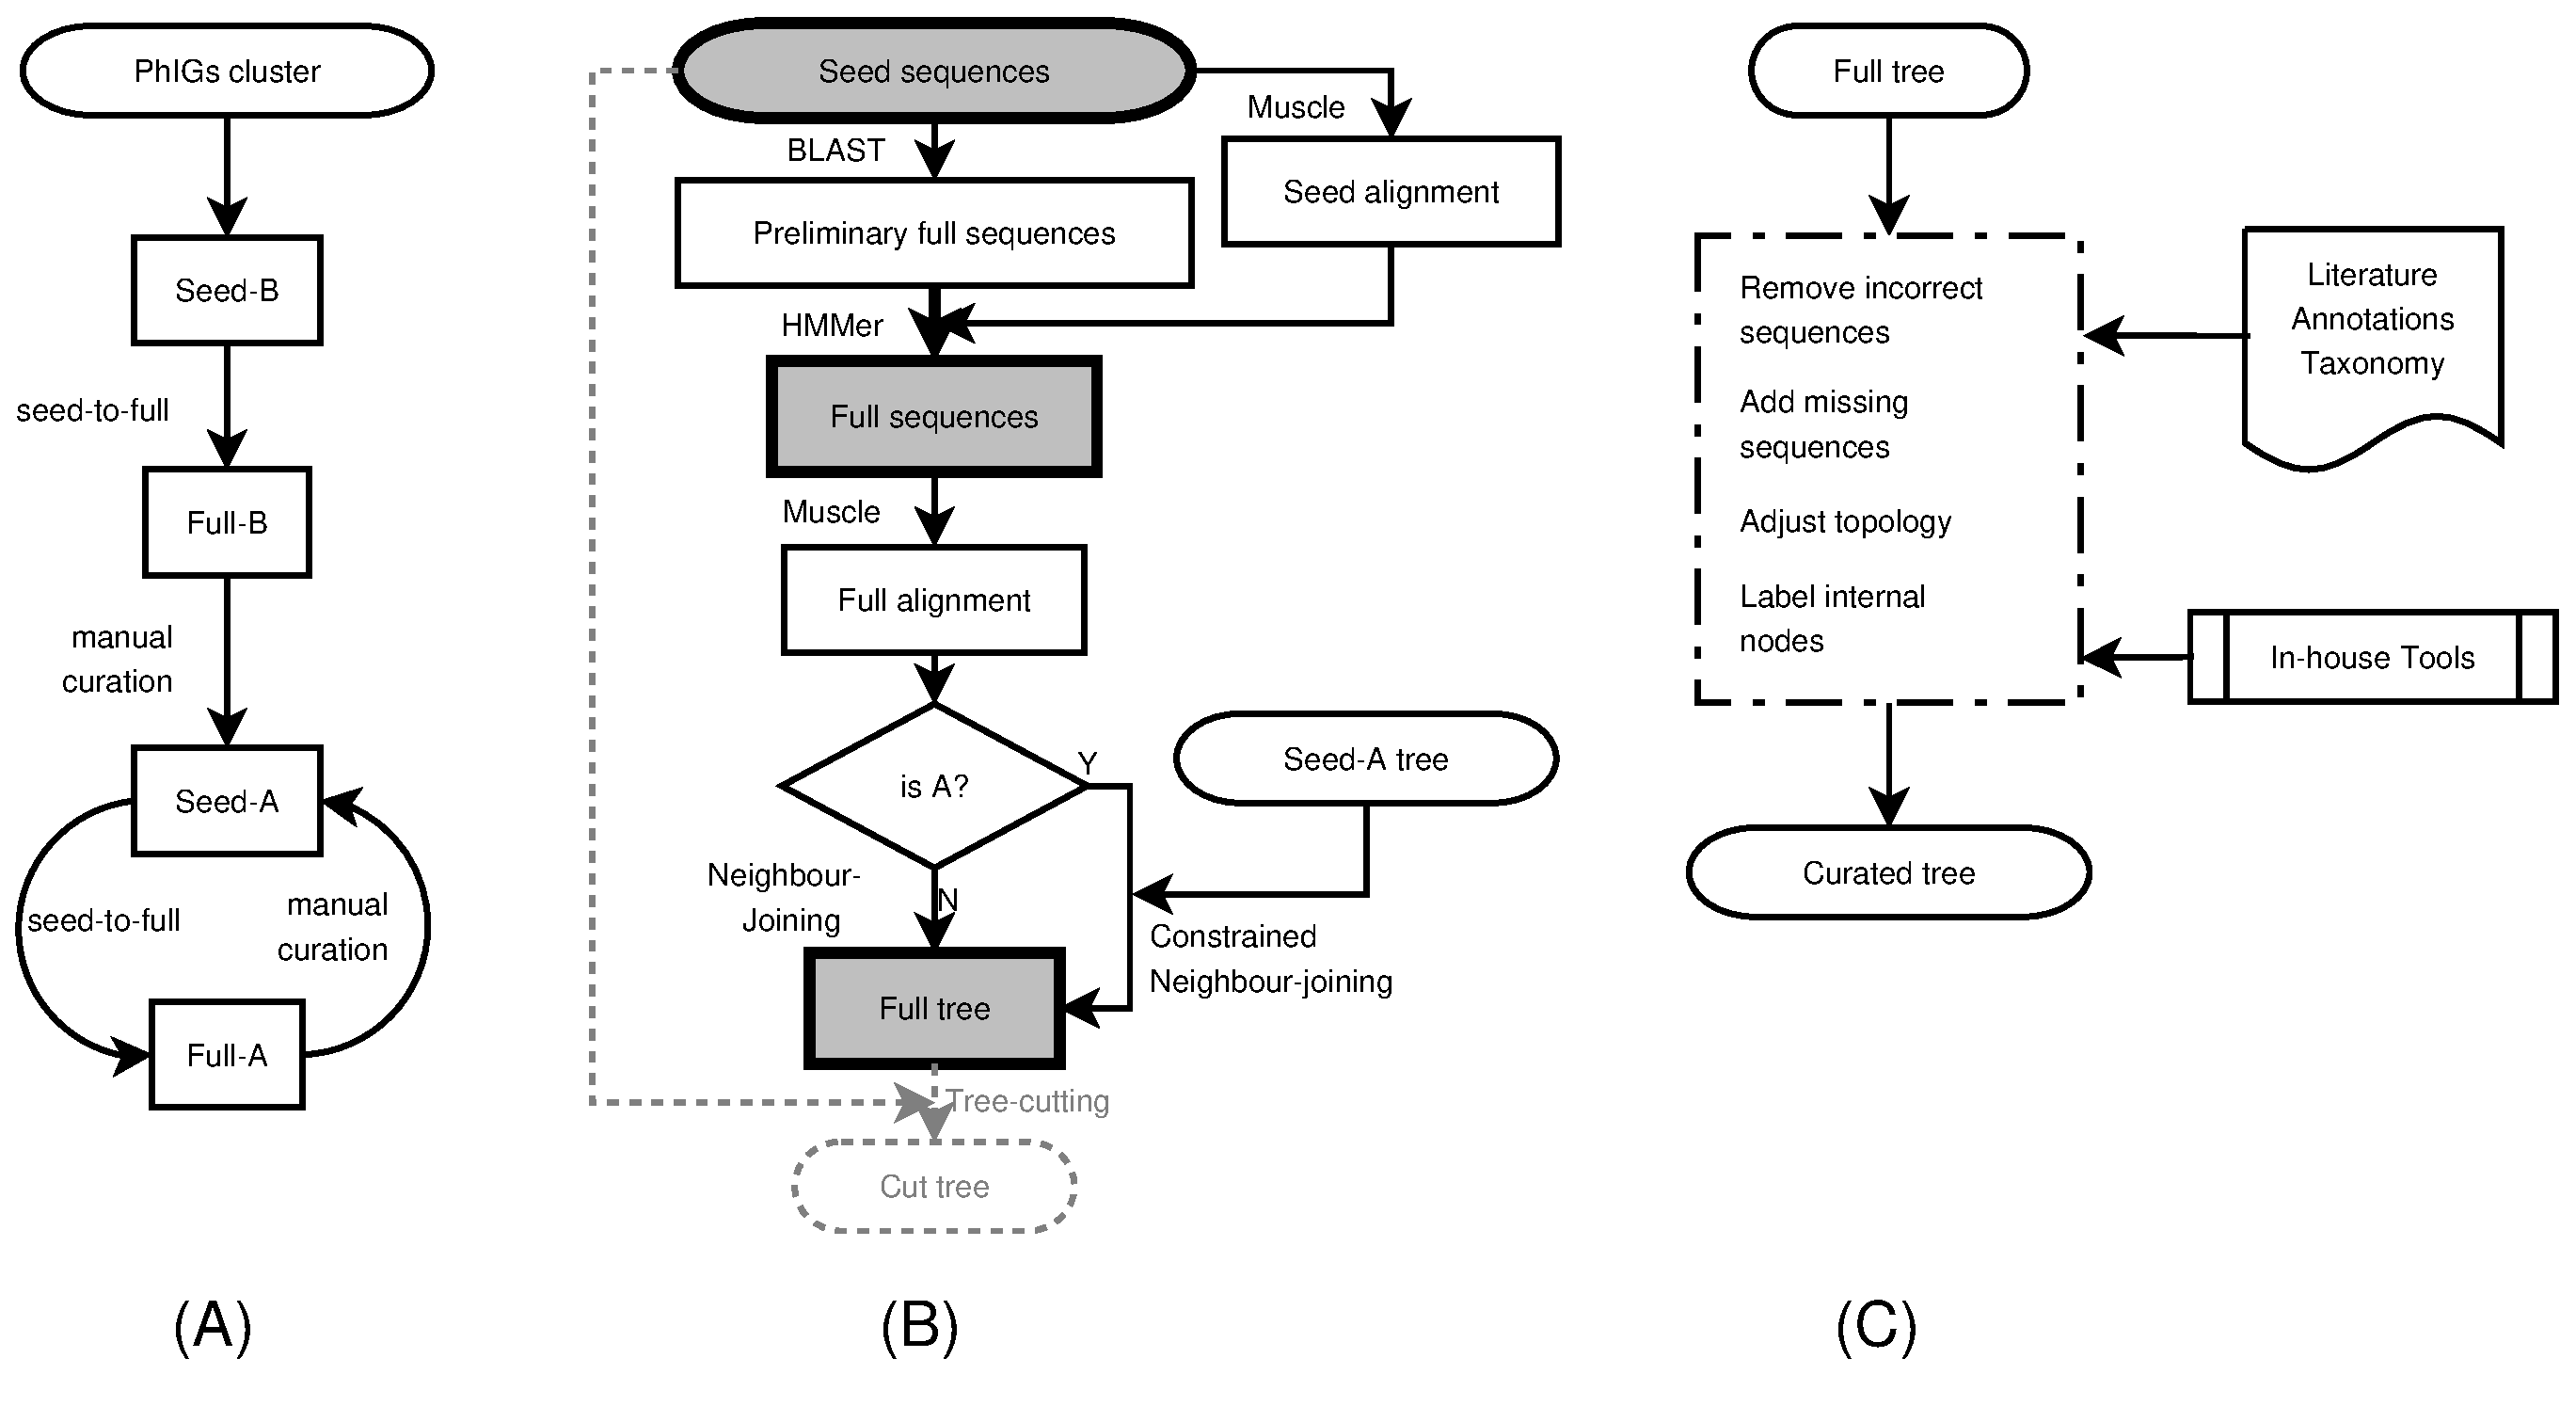
\includegraphics[width=\textwidth]{flowchart}
\caption[Flowchart of TreeFam pipeline]{Flowchart of TreeFam pipeline. (A) Overall strategy. The seed
  families for TreeFam-B are taken from PhIGs clusters. They are expanded by a seed-to-full procedure
  to form full families. Manual curation makes TreeFam-B families become TreeFam-A families, which can
  also be curated further at a later date. (B) The seed-to-full procedure. Dashed lines and gray texts show
  the actions only present in TreeFam-1.x. In the boxes with gray background, details have been changed since
  TreeFam-2. Seed-to-full procedure is used to expand seed sequences to full sequences. Note that
  the complete procedure is only applied when the sequences sets are updated or a whole new genome
  is added to TreeFam. For TreeFam-A families created by curation of a TreeFam-B families,
  the TreeFam-A seed is generated by manual curation, and the full sequences are taken directly
  from the TreeFam-B that was curated. (C) Manual curation. Various published resources and in-house tools
  are utilized in this process.}\label{fig:flowchart}
\end{figure}

\section{Input Data}
\subsection{Sequence data}
TreeFam 2.0 collected protein and coding sequences for 19 fully sequenced species from GenBank~\cite{wheeler05},
SGD~\cite{balakrishnan05}, WormBase~\cite{chen05}, GeneDB~\cite{hertzfowler04} and
Ensembl~\cite{hubbard05} (Table~\ref{tab:species}).
Protein sequences for species that have not
been sequenced were obtained from UniProt~\cite{bairoch05}. Genomic locations and Pfam~\cite{bateman04} domain
structures of genes were also included if available. In this chapter, TreeFam sequence set will be called
TFSEQ\index{TFSEQ} for simplicity.

Of the 19 species, two yeasts and {\it A.thaliana} serve as outgroup species. In a gene tree, genes of outgroup speices
help to reveal ancestral species earlier than the LCA of metazoan animals, and thus indicate
when two groups of animal genes should belong to two TreeFam gene families instead of one.
Outgroups set the boundaries of gene families.

\begin{table}[!hb]
\begin{center}
{\tt
\begin{tabular}{|r|l|l|l|}
\hline
Tax ID & Tax Name & {\it abbr.}	& Common Name\\
\hline
9606	& {\it Homo sapiens}				& HUMAN & Human\\
9598	& {\it Pan troglodytes}				& PANTR & Chimpanzee\\
10090	& {\it Mus musculus}				& MOUSE & Mouse\\
10116	& {\it Rattus norvegicus}			& RAT 	& Rat\\
9615	& {\it Canis familiaris}			& CANFA & Dog\\
9031	& {\it Gallus gallus}				& CHICK & Chicken\\
8364	& {\it Xenopus tropicalis}		& XENTR & Western clawed frog\\
31033	& {\it Fugu rubripes}			& FUGRU & Japanese pufferfish\\
99883	& {\it Tetraodon nigroviridis}	& TETNG & Green puffer\\
7955	& {\it Danio rerio}				& BRARE & Zebrafish\\
7719	& {\it Ciona intestinalis}		& CIOIN & \\
7227	& {\it Drosophila melanogaster}	& DROME & Fruit fly\\
7165	& {\it Anopheles gambiae}		& ANOGA & African malaria mosquito\\
7460	& {\it Apis mellifera}			& APIME & Honeybee\\
6239	& {\it Caenorhabditis elegans}	& CAEEL & \\
6238	& {\it Caenorhabditis briggsae}	& CAEBR & \\
4896	& {\it Schizosaccharomyces pombe}	& SCHPO & Fission yeast\\
4932	& {\it Saccharomyces cerevisiae}	& YEAST & Baker's yeast\\
3702	& {\it Arabidopsis thaliana}		& ARATH & Mouse-ear cress\\
\hline
\end{tabular}
}
\caption[Fully sequenced species that are included in TreeFam-2]
{Fully sequenced species that are included in TreeFam-2. Two yeasts and {\it A.thaliana} serve
as outgroup species that are used to indicate the boundary of a gene family.}~\label{tab:species}
\end{center}
\end{table}

\subsection{Original seeds}
The start point of the entire TreeFam pipelines is the construction of seeds of TreeFam-B families,
which has to be achieved by clustering methods. Fortunately, PhIGs has already done this
in the way we desired. In PhIGs, clusters are inferred to have descended from
a single gene from the last common ancestor of a specified group of species.
Genes are grouped together following the evolutionary relations between species, instead of
sheer similarity scores.
At present, two types of clusters are presented in PhIGs website: one for all vertebrates,
and the other for all metazoan animals. Ideally, a gene cluster of the latter type is exactly equivalent
to a gene family defined in TreeFam, and therefore TreeFam skips the clustering step
and directly uses PhIGs clusters as the original seed sets.

\subsection{Miscellaneous data}
A phylogenetic tree not only presents the history of a gene family. It also
provides the basis for various evolutionary researches, such as studies related to
intron evolution, domain evolution, and shift of gene functions. To help
these studies and to discover the principles behind evolutionary phenomena,
we also integrate several other resources with TreeFam. Since TreeFam-2.0, splicing
information and domain structures of each gene have been available.
Expressional profiles of genes will be provided in TreeFam-3. Phenotypes from
a knockout screen and GO ontology~\cite{ashburner00} categories may also be considered
in future.

\section{Automatic Pipelines}
Pipelines used for constructing TreeFam 2.0 mainly differ from those for 1.x
in two aspects: grouping of PhIGs clusters and use of the competitive method.
As TreeFam paper has already presented detailed procedures used in 1.x series,
we only focus on the 2.0 pipelines in this section.

\subsection{Generating seeds of TreeFam-B families}
In TreeFam release 1.x series, PhIGs clusters that consisted of three or more vertebrate sequences were
directly used as the seeds of TreeFam-B families. However, as PhIGs seemed to apply
a very stringent threshold at clustering stage, it sometimes split a gene family
into several smaller clusters if family members were too divergent.
This has been observed at times in curation processes, and made us
consider clustering PhIGs results when TreeFam 2.0 was planned.

Since TreeFam 2.0, PhIGs clusters are grouped as follows. First, sequences of original clusters
are aligned against TFSEQ by BLAST\footnote{BLAST (Basic Local Alignment Search Tool)
is the most popular alignment program that finds the homologs of one sequence.
It aligns one sequence against each sequence in a sequence set and measures the similarity
by an alignment score. Then BLAST evaluates the significance 
of homology by E-value which is the mathematical expectation of the number of sequences having scores higher than the observed score
when a random sequence is aligned against a random sequence set of the same size.}~\cite{altschul97}
with E-value cutoff $0.01$.
Matched TFSEQs are searched again by HMMER\footnote{HMMER is also a tool for homolog search. It builds an HMM (hidden Markov model)
profile based on a multialignment. It then makes use of the profile to measure how well
a sequence matches the given multialignment. Utilizing a set of sequences, HMMER
is more sensitive and more accurate than BLAST which only performs pairwise alignment.
However, HMMER is much slower than BLAST.}~\cite{eddy98} with E-value cutoff $0.1$.
HMM profiles in this step are built from MUSCLE\footnote{MUSCLE is a multialignment
program like Clustalw. It puts all sequences together and aligns them such that their
homologous regions match with each other. Generally, MUSCLE is much faster and more accurate than
Clustalw~\cite{edgar04}.}~\cite{edgar04} multialignments of original
PhIGs clusters. A relational graph is then constructed from HMMER results. In this graph,
each vertex is an original PhIGs cluster. A weighted edge is added if the HMMER
results of two clusters share some animal genes. More precisely,
given a PhIGs cluster $u$, let $R_u$ be the set of TFSEQ animal genes whose HMMER bit-score
are higher than scores of any outgroup genes matched by sequences in $u$. An edge is added between
two clusters $u$ and $v$ if $R_u\cap R_v\not=\emptyset$. The weight of this
edge is $\frac{|R_u\cap R_v|}{\min\{|R_u|,|R_v|\}}$. After the construction
of this weighted graph, clustering can be achieved by various means
based on graph theory. In TreeFam 2.0, we implemented a heuristic algorithm
revised from Zdobnov {\it et al.}~\cite{zdobnov02}. Like most similar methods, this algorithm tries to find groups
in which edges tend to be saturated~\footnote{As a matter of fact, MCL algorithm~\cite{enright02}
is more sophisticated in this case.}. Finally, grouped PhIGs clusters are
merged to form a larger one, which is regarded as a new cluster in next round.
In theory, this grouping process should be iterated for many times until the results
are stable, but in practice we found that grouping two or more times will
lead to many superfamilies that contain several animal families, seemingly due to the reason that HMMER becomes
insensitive when clusters get larger. Consequently, only one round of
grouping is applied. The results are then used as the seeds of TreeFam-B families.

\subsection{Competitively assigning each sequence to one family}
In TreeFam 1.x, family members were determined by tree cutting algorithm. This algorithm
discarded homologs that are descendants of a different (paralogous) gene in
the last common ancestor of animals. Ideally, such a behaviour is exactly what we desired.
However, due to the tendency of missing distant homologs and the difficulties
in reconstructing long branches, tree cutting malfunctioned at times and resulted
in families that consisted of excessive members. Thus in TreeFam 1.x, one gene
could belong to several or even dozens of families, which by itself was inconsistent and
also caused much trouble in curation. In addition, as multialignments and phylogenetic trees had to be built
before unnecessary sequences were discarded, huge multialignments that contained
over 500 genes were encountered from time to time, which greatly
aggregated computational burden. Consequently, we decided to develop a
better strategy to assign sequences to TreeFam families.

In TreeFam-2.0, homologous sequences are still collected by a combination of BLAST and HMMER:
homologs are first found by BLAST and then refined by HMMER with the profile built from
seed multialignment by MUSCLE. After this step, one sequence
is competitively assigned to one family which gives the
sequence the highest HMMER score; if one family contains several splicing forms of one
gene, only the transcript with the highest HMMER score is retained. Family members
are determined at this time.

To our observations, HMMER usually works quite well if the quality of seeds is
high enough. Most of animal genes, especially vertebrate genes, can be
correctly assigned in this way. However, when seed contains few sequences or
the seed alignment is too poor, HMMER score will be inaccurate and
cause errors. Furthermore, the existence of orphan genes and the
incompleteness of the whole seed set also interfere. Even if a gene does not
belong to any existing TreeFam families, it will still be forcedly assigned
no matter how low the BLAST and HMMER scores are. In the next release of TreeFam,
this problem will be paid more attention.

\subsection{Tracing sequence identifiers for TreeFam-A families}
TreeFam stores curated knowledges in TreeFam-A seed trees. However, with the update
of sequence sets, genes in previous seed trees might be absent in the latest sequence sets when
the identifiers have been changed. In this case, some curation cannot be reserved, and loss of
of information occurs. And continuous loss of information will finally wipe
out all the effort in curation. To slow down this process is very important to a curated
database like TreeFam.

In TreeFam-2.0, a particular pipeline is designed to trace sequence identifiers when they are changed
between releases. The basic idea is to map a new identifier to an old one if~\footnote{These rules
will be changed since TreeFam-3.0.}: (i) the two
sequences come from the same species; (ii) the two are almost identical in matched regions;
and (iii) no other sequence is closer to either of the two sequences. The condition (i) and (ii)
are obvious and can be easily judged. The third condition can be tested by studying the
tree that consists of both unchanged sequences and sequences whose identifiers
are only present in one release, either old or new. In this tree, condition (iii) is satisfied if
a new identifier and an old one share the same parent node. Figure~\ref{fig:exam-traceid} shows
an example where violation of condition (ii) and (iii) occurs.

\begin{figure}[!hb]
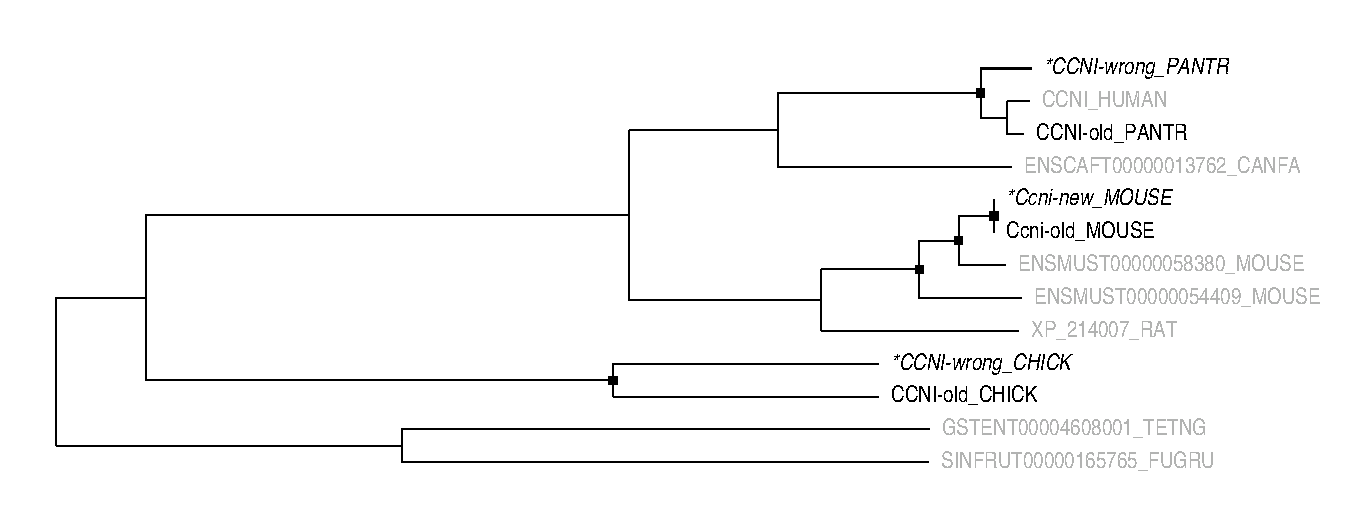
\includegraphics[width=\textwidth]{traceid}
\caption[Example explaining trace-ID procedure]{Example explaining trace-ID procedure. This tree consists of both
unchanged sequences (in gray) and sequences whose identifiers differ between releases (in black).
Sequences only present in the new release are highlighted in slanting font.
Identifier {\tt CCNI-old\_PANTR} shall not be mapped to {\tt *CCNI-wrong\_PANTR}
because {\tt CCNI\_HUMAN} is closer to the former one (violating (iii)).
ID {\tt CCNI-old\_CHICK} cannot be mapped to {\tt *CCNI-wrong\_CHICK} because
they are not close enough (violating (ii)) although they share the same parent node.
Only the two mouse genes can be mapped.
}\label{fig:exam-traceid}
\end{figure}

\subsection{Building trees}
With irrelevant distant homologs discarded in TreeFam-2 families, family trees are much smaller than those in
TreeFam-1.x, which makes it possible to reconstruct trees with more accurate, yet
slower, algorithms such as maximum-likelihood methods. In addition, tree merge algorithm (Chapter~\ref{chap:merge})
is also applied more frequently, and further improves the quality of phylogenetic trees.

In the new TreeFam-B, a full tree is reconstructed, at protein level, by neighbour-joining constrained (Section~\ref{sec:cnj})
by $d_m$ tree, the synonymous-nonsynonymous merged tree. In TreeFam-A, full trees are further required to be constrained by seed trees.
While tree reconstruction at protein level gets more sequences involved,
the use of synonymous tree improves the topologies at lower branches.
In the effort to build even better automatic trees, we also build a `clean tree' that is merged
from four trees including ML protein tree, ML nucleotide tree, NJ synonymous tree and
NJ nonsynonymous tree (Chapter~\ref{chap:merge}). This method really outperforms
all the others both in our benchmark and to our experience in manual curation processes (Chapter~\ref{benchmark}).

\chapter{Reconstructing Gene Trees} \label{chap:buildtree}

Phylogenetic trees represent the history of evolution instead of measuring the similarity
between sequences. Since the history can never be changed, correct trees are always there.
Good algorithms must correctly recover the history.
On the other hand, as no one knows what exactly happened in history, phylogenetic trees
have to be reconstructed based on present observations. While fossils are essential
evidence to reconstruct species trees, reconstructing gene trees can only utilize
sequence similarity because fossils are usually insufficient and unable to date
molecular events. Consequently, how to precisely recover the true history from sequence similarity
becomes the eternal topic in evolutionary studies.

This chapter is to describe how TreeFam reconstructs a gene tree provided a multialignment.
After an overview of various tree-building algorithms\index{tree building algorithm}, constrained neighbour-joining,
one of the exceptional algorithms developed in TreeFam, will be presented.
Rooting a tree will be discussed in the next.
Bootstrapping test and leaves reordering algorithm are also introduced here because the two
topics are closely related to tree building process. In TreeFam-1.x, neighbour-joining is
the only algorithm we used to build trees, but since the release of TreeFam 2.0,
more sophisticated algorithms, including maximum-likelihood method and tree merge, are applied.
These methods are not covered in this chapter, but are discussed in Chapter~\ref{chap:merge} and evaluated
in Chapter~\ref{chap:benchmark}.

\section{Overview of Tree Building Algorithms}

Whereas phylogenetic trees can be reconstructed with various evolutionary characters,
molecular phylogenetics mainly focuses on tree reconstruction from multiple-sequence
alignments. Throughout this thesis, multialignment is the starting point of tree reconstruction.
Most of algorithms discussed in this thesis will take a multialignment as the unique input.
Only in Chapter~\ref{chap:merge}, auxiliary information will be integrated with tree building process.

Tree building algorithms can be classified into four types: distance based, parsimonious,
maximum-likelihood, and Bayesian methods. Each type of algorithm has its own strength and
weakness. In meticulous case studies, all kinds of algorithms should be tried in attempt
to reconstruct a reliable phylogenetic tree. This has been confirmed by the benchmark
done in Chapter~\ref{chap:merge}.

\subsection{Distance based algorithms}
Distance based method is actually the name of a group of algorithms that reconstruct a tree
from a distance matrix $(d_{ij})$ where an element $d_{ij}$ measures a kind of distance
between sequence pair $i$ and $j$. Distances are usually, though not necessarily,
calculated from a multialignment. They can be alignment scores, number of mismatches
(also called p-distance), or historical substitution frequencies estimated from
statistical models.

Of all distance based algorithms, UPGMA~\cite{sokal58}\index{UPGMA} is the earliest. It
mimics hierarchical clustering processes, joining the pair of closest nodes. UPGMA assumes
the divergence of sequences occurs at a constant rate at all branches (molecular clock), which, unfortunately,
does not always stand. Lateral algorithms do not arbitrarily require this hypothesis any longer,
though the existence of a molecular clock help to improve the accuracy of tree building.
In 1967, Cavalli-Sforza and Edwards~\cite{cavalliSforza67}
suggested that tree can be built such that the length of the path between any leaf pair in the tree
should approach the distance given by the distance matrix. This gave the rise
of LS (least square)\index{LS, least square} method. The reconstruction of a LS tree
require to search the whole tree space for the optimal tree, which is formidable.
Thus, Fitch and Margoliash~\cite{fitch67}\index{Fitch-Margoliash}
further simplified this procedure and presented a algorithm that was practically useful.
The breakthrough came in 1987 when Saitou and Nei~\cite{saitou87} invented NJ (neighbour-joining)
algorithm. Instead of joining a pair of closest nodes at each step like UPGMA, NJ joins a neighbour and
does not assume the existence of a molecular clock.
It is simple, accurate and efficient. Two alternatives, BIONJ~\cite{gascuel97}\index{BIONJ} and
Weighbor\index{Weighbor}~\cite{bruno00}\index{Weighbor}, were also developed by improving the joining procedures.
As a matter of fact, neighbour-joining is a greedy approximation of ME (minimum
evolution\footnote{Minimum evolution (ME) principle regards that nature favours the tree with minimum
sum of the lengths of the branches. In some way, it resembles maximum parsimony principle
introduced in next subsection. Rzhetsky and Nei~\cite{rzhetsky93}
prooved that ME tree is correct `provided that the evolutionary distances used are statistically
unbiased and that the branch lengths are estimated by the ordinary least-squares method'.})~\cite{rzhetsky93}.
It follows ME rule at each separated step, but does not build a true ME tree.
Recently, Desper and Gascuel~\cite{desper04} developed
BME framework (balanced minimum evolution)\index{BME, balanced minimum evolution}
where ME tree can be precisely reconstructed.
Their program FASTME\index{FASTME} was claimed to be both faster and more accurate than NJ and
all its offshoots, which is partly confirmed in Chapter~\ref{chap:benchmark}.

Distance based method is popular mainly for its unparalleled speed. It is the only
hope for reconstructing a phylogeny containing as many as 1000 sequences. However, distance method
is always criticized for its loss of information: substitutions on
each site between two sequences are compacted into a single number. This
compression not only affects the accuracy, but also limits the further application.
For example, it is not allowed to reconstruct ancestral sequences, or
to estimate evolutionary parameters such as transition/transversion ratio and $\Gamma$ rate
in the distance based framework. In those cases, we must fall back
to other methods.

\subsection{Maximum parsimony}
Given a phylogenetic tree and a multialignment, we can trace back the history
presented by the tree and calculate the minimum number of substitutions that are required
to explain the given data. Different trees usually yield different numbers.
MP (Maximum parsimony) algorithm~\cite{fitch71}\index{MP, maximum parsimony}
works by searching the whole tree space for the tree that minimizes the minimum number of substitutions.

Based on the principle of Ockham's
razor~\footnote{Given two equally predictive theories, choose the simpler,
and the simplest answer is usually the correct answer. {\it See also}
\href{http://en.wikipedia.org/wiki/Occam's\_Razor}{http://en.wikipedia.org/wiki/Occam's\_Razor}.},
MP algorithm is most appealing for its simplest
assumption: a true tree tends to contain fewer substitutions.
No evolutionary model is in need to build a parsimonious tree.
While this advantage attracts many biologists, statistists see it in a different way.
They criticized that MP is unable to reconstruct a correct tree when long branches appear~\cite{felsenstein78}.
They argued that MP is actually based on an irrealistic model where substitutions occur
uniformly both across sites and across subtrees~\cite{holder03}.
They claimed that MP yields less information in comparison to
max-likelihood methods. However, although being faced with these long-lasting disputes, MP
remains popular and shows its power especially for close homologs.

\subsection{Maximum-likelihood and Bayesian methods}
ML (maximum-likelihood) method~\cite{felsenstein81} finds the tree that maximizes the likelihood
given a specified evolutionary model. Regardless of efficiency issues, the procedure of ML reconstruction
is very simple: calculating the likelihood and finding the best tree.
While ML method presents the theoretical framework, its power is actually
determined by statistical models, which also makes ML method
very versatile due to the flexibility of models.
Various evolutionary information can be smoothly inferred in the statistical framework.
ML method is definitely the most fruitful method of all the tree building algorithms.
Furthermore, ML method was also claimed to be the
most accurate tree building algorithms in several studies~\cite{kuhner94,hall05}.
Most of molecular evolutionists will agree that the use of ML method reformed the system of phylogenetics.

However, applying ML method is extremely computation extensive. Even when a number of heuristic
algorithms were designed to accelerate tree searching~\cite{olsen94,guindon03,stamatakis05}, building
a tree with hundreds of leaves is still formidable, not to speak
bootstrapping the alignment (Section~\ref{sec:bootstrap}).
In addition, although ML method allows for various evolutionary models in use, these models have to
be preset in softwares and cannot be combined at will. This affects its further use
in complex phylogenies.

Bayesian method can be regarded as an alternative to ML method. But instead of actively traversing the whole
tree space to find the one with maximum likelihood like ML, it finds the one that maximizes posterior probability
by sampling phylogenetic trees through MCMC (Markov Chain Monte Carlo) based on the specified model~\cite{rannala96}.
The most exciting advantage of Bayesian method is its unparalleled flexibility. As
it just generates trees instead of calculating the probability of a given tree, complex analytical computations
can be avoided. Thus, various complex models can be easily designed and combined together, and
by summarizing from a bulk of sampled trees,
parameter estimation also becomes painless. Furthermore, sampled trees in MCMC process
can be considered as resampled trees to some extend~\cite{larget99}. Support values are naturally calculated
with less computational resources, though these values may be `excessively high' as pointed out
by several works~\cite{suzuki02,cummings03,simmons04}.

\section{Constrained Neighbour-Joining} \label{sec:cnj}

All traditional tree-building algorithms are unsupervised in that they never make use of
additional knowledge provided by a human. Even if we know a leaf set $A$ should be
separated from $B$, they can be still mixed up in the resultant tree. In TreeFam,
however, we must preserve the topology of the seed tree, or the knowledge of curators, when building a full tree.
This is a supervised procedure. New algorithm must be designed for this goal; otherwise
the effort of curation would come to naught when the full tree does not utilize
the curated topology. In this section we introduce the first key algorithm of TreeFam,
constrained neighbour-joining (cNJ), which can add new sequences to an existing tree
without changing the given topology. We start with the standard neighbour-joining.

\subsection{Standard neighbour-joining algorithm}
A distance matrix is said to be \emph{additive}\index{additive} if there exists a binary tree from which
the length of the path~\footnote{In a tree, the path length equals to the sum of lengths of the edges/branches in the path.}
connecting each pair of leaves equals to
the their pairwise distance presented by the matrix. In turn, if a distance matrix is additive, we can
always reconstruct the tree that makes the additivity. Neighbour-joining~\cite{saitou87}
is the algorithm that finds this tree.

Neighbour-joining works by adding a new internal node that joins a pair of neighbouring leaves at each step.
Given a symmetric distance matrix $(d_{ij})_{n\times n}$, a neighbour pair is the pair of leaves that minimizes $D_{ij}$ of
all possible $(i,j)$, where $D_{ij}$ is defined as:
\begin{eqnarray*}
D_{ij}&=&d_{ij}-(r_i+r_j) \\
r_i&=&\frac{1}{n-2}\sum_{k=1}^n d_{ik}
\end{eqnarray*}
When a new node $K$ is added to join a neighbour $(I,J)$, the distances between them
can be calculated as:
\begin{eqnarray*}
d_{IK}&=&\frac{1}{2}(d_{IJ}+r_I-r_J) \\
d_{JK}&=&d_{IJ}-d_{IK}
\end{eqnarray*}
And the distances between $K$ and all the other nodes are:
\[
\mbox{$d_{Km}=\frac{1}{2}(d_{Im}+d_{Jm}-d_{IJ})$, for $m=1,2,\ldots,n$, $m\not=I$ and $m\not=J$}
\]
With neighbour $I$ and $J$ removed and $K$ added, the original $n\times n$ distance matrix $(d_{ij})$ will be reduced
to $(n-1)\times(n-1)$. This finishes one round of iteration. When this process is applied
repeatedly until the matrix becomes $3\times3$\footnote{This is because in an unrooted binary tree each internal node
has three edges attached.}, the three remaining nodes should be
joined together. Tracing the joins at each step we can make a binary unrooted tree,
which is the standard neighbour-joining tree.
If the distance matrix is additive, this tree suffices additivity.
Proof can be found in the book written by Durbin {\it et al.}~\cite{durbin98}.

Neighbour-joining algorithm joins the pair that minimizes $D_{ij}$ instead of $d_{ij}$.
This is one of the main points where neighbour-joining differs from UPGMA algorithm.
Minimizing $D_{ij}$ can avoid false-joining when long branches occur, and the existance
of long branches will always break the molecular clock, which will fail UPGMA.
This is the strongth of neighbour-joining.

\subsection{Constrained neighbour-joining algorithm}
The basic idea of neighbour-joining algorithm is very simple. The only difference between
the standard neighbour-joining and the constrained one is that
constrained neighbour-joining disallows joining that are conflict with the topology of
the given constraining tree. As in each step all pairs of leaves will be checked, check of valid
joining must be fairly efficient. As a matter of fact, if we notice the fact that joining
is only allowed between two leaves with the same parent node,
we can contract the constraining tree by removing joined leaves and making the parent a new
external node. Such contract is performed each time when two leaves in the constraining tree
are joined together. As checking whether two leaves sharing a same parent
can be done in $O(1)$, validating allowed joining can also be achieved in $O(1)$ time, and consequently,
constrained neighbour-joining has the same time complexity with that of the original one,
that is, $O(N^3)$ where $N$ is the number of leaves.
Figure~\ref{fig:example-cnj} also gives an example.
Detailed algorithm is described in Table~\ref{tab:cnj}. This table also
presents the standard neighbour-joining algorithm.

\begin{figure}[!hb]
\begin{center}
\includegraphics{mpfig.9}
\caption[Example of constrained neighbour-joining algorithm]
{Example of constrained neighbour-joining algorithm. In the first three rows, the left is the
constraining tree at current step; the right shows the remaining nodes and the best allowed joining.
At step 3, only three nodes remains. They are joined together, which makes a trifurcation. The resultant
tree is showed in the end. Note that no constraint is applied to node `3'. It can be freely joined to other
if node `3' neighbours a certain node at some step.}\label{fig:example-cnj}
\end{center}
\end{figure}

\begin{table}[!hb]
\begin{center}
\begin{tabular}{|ll|}
\hline
&\textbf{Input:} \\
&\lhspace Distance matrix $(d_{ij})$ \\
&\lhspace A rooted constraining tree $C$ with all its leaves appearing in the matrix \\
&\textbf{Output:} \\
&\lhspace A neighbour-joining tree $T=(V(T),E(T))$ \\
&\textbf{Procedure:} \\
&\lhspace Let $\mathcal{L}$ be the set of nodes that appear in the distance matrix \\
&\lhspace$\mathcal{L}_C\gets V_E(C)$ \\
&\lhspace$V(T)\gets\mathcal{L}$ \\
&\lhspace$E(T)\gets\emptyset$ \\
&\lhspace\textbf{while} $|\mathcal{L}|>3$ \textbf{do} \\
&\lhspace\lhspace{\bf for} each node $i\in\mathcal{L}$ {\bf do} \\
&\lhspace\lhspace\lhspace$r_i\gets\frac{1}{|\mathcal{L}-2|}\sum_{k\in\mathcal{L}}d_{ik}$ \\
&\lhspace\lhspace$M\gets\infty$\\
&\lhspace\lhspace{\bf for} each node pair $(i,j)\in\mathcal{L}\times\mathcal{L}$ {\bf do} \\
&\lhspace\lhspace\lhspace$D_{ij}\gets d_{ij}-(r_i+r_j)$\\
&\lhspace\lhspace\lhspace\textbf{if} $D_{ij}<M$ \textbf{then} \\
$\ast$&\lhspace\lhspace\lhspace\lhspace{\bf if} $\{i,j\}\not\subset\mathcal{L}_C$ {\bf OR} $\lhparent_C(i)=\lhparent_C(j)$ {\bf then} \\
&\lhspace\lhspace\lhspace\lhspace\lhspace$M\gets D_{ij}$, $I\gets i$ and $J\gets j$ \\
&\lhspace\lhspace$V(T)\gets V(T)\cup\{K\}$\\
&\lhspace\lhspace$E(T)\gets E(T)\cup\{(K,I)\}\cup\{(K,J)\}$\\
&\lhspace\lhspace{\bf for} each node $m\in\mathcal{L}$ {\bf do}\\
&\lhspace\lhspace\lhspace$d_{Km}\gets\frac{1}{2}(d_{Im}+d_{Jm}-d_{IJ})$\\
&\lhspace\lhspace$d_{IK}\gets\frac{1}{2}(d_{IJ}+r_I-r_J)$ \\
&\lhspace\lhspace$d_{JK}\gets d_{IJ}-d_{IK}$ \\
&\lhspace\lhspace$\mathcal{L}\gets\left(\mathcal{L}\cup\{K\}\right)\setminus\{I,J\}$ \\
$\ast$&\lhspace\lhspace\textbf{if} $\{I,J\}\cap\mathcal{L}_C\neq\emptyset$ \textbf{then} \\
$\ast$&\lhspace\lhspace\lhspace\textbf{if} $\lhchild(\lhparent_C(I))=\{I,J\}$ \textbf{then} \\
$\ast$&\lhspace\lhspace\lhspace\lhspace$\lhparent_C(K)\gets\lhparent_C(\lhparent_C(I))$ \\
$\ast$&\lhspace\lhspace\lhspace\textbf{else if} $I\in\mathcal{L}_C$ \textbf{then}\\
$\ast$&\lhspace\lhspace\lhspace\lhspace$\lhparent_C(K)\gets\lhparent_C(I)$ \\
$\ast$&\lhspace\lhspace\lhspace\textbf{else if} $J\in\mathcal{L}_C$ \textbf{then}\\
$\ast$&\lhspace\lhspace\lhspace\lhspace$\lhparent_C(K)\gets\lhparent_C(J)$ \\
$\ast$&\lhspace\lhspace\lhspace$\mathcal{L}_C\gets\left(\mathcal{L}_C\cup\{K\}\right)\setminus\{I,J\}$ \\
&\lhspace add a new node $K$ that joins the remaining three nodes in $\mathcal{L}$ \\
\hline
\end{tabular}
\caption[Algorithm for constrained neighbour-joining]
{Algorithm for constrained neighbour-joining. Lines labeled by `$\ast$' are specific to
constrained neighbour-joining. By removing these lines, we can get the ordinary NJ algorithm.}\label{tab:cnj}
\end{center}
\end{table}

\subsection{Further discussion}
As a matter of fact, constrained neighbour-joining presented above does not follow the neighbour-joining rule.
It cannot ensure that an allowed pair of neighbours can always be joined. This is because constrained NJ
assumes the constraint is a rooted tree. It will not consider other rooted topologies and
arbitrarily join the nodes in the suffix order\footnote{If the nodes of a rooted tree are traversed in suffix order,
lower nodes will always be visited earlier than higher nodes.}
of the given constraining tree.
 To explain this, let's see an example. Assume we have a tree
{\tt ((1,2),3,4)} reconstructed by standard NJ. From the given tree, the only joining happens
between leaf {\tt 1} and its neighbour {\tt 2}. Now, we continue to assume that the
rooted topology of this tree should be {\tt (((3,4),2),1)} and use this rooted
tree as constraint. Then {\tt (3,4)} must be joined first by constrained NJ described above, although
the true neighbour {\tt (1,2)} does not violate the constraint in the unrooted topology.
Constrained NJ shuffles the order of joining and breaks NJ rule.

If the distance matrix was strictly additive, or equivalently, if the distance between any pairs of
the leaves always equaled to the length of the path that connects the pair,
the order of joining would be unimportant. Joining in any order will lead to the same tree, including the branch length.
In the real world, however, strict additivity is rarely held. Even if a standard NJ
is used as constraint, constrained NJ will frequently generate a tree with different
branch length, though the topology is the same.

Given this fact, we also developed another version of constrained neighbour-joining that
regards the constraint as an unrooted tree. On the example above, the new version
will correctly join the neighbour {\tt (1,2)} in the first step. This is also an $O(N^3)$ algorithm, but it
can only be applied when the constraint is a binary tree; otherwise the time complexity will
be increased. This algorithm is much more complex than the previous one and will not be described in this thesis.

\section{Rooting Trees} \label{sec:root-tree}
Any phylogenetic tree is a rooted tree given the hypothesis that all organisms on Earth
had a common ancestor. However, neighbour-joining and likelihood method can only reconstruct
an unrooted tree, and so algorithms must be developed to root a tree. In fact, rooting is of the same
importance as building a tree. A wrong root leads to a different story.

There are several ways to root a tree. The most widely used one is to select an outgroup sequence
among all the leaves, and directly put the root on the branch that connects the outgroup. However,
in lack of adequate biological evidence, outgroups are hard to decide especially for some complex gene families.
It is impossible to automatically define an outgroup for every TreeFam family, and so
this method is not applicable to TreeFam.

Another method is to minimize the height among all the possible rooted trees, which can be achieved by
placing the root at the middle point of the longest chain of consecutive edges.
It works well if deviations from molecular clock is not that much~\cite{durbin98}.
This method was further extended in Bayesian framework~\cite{huelsenbeck02}.

A more sophisticated method, the one used by TreeFam, is to minimize the
dissimilarity between the gene tree and a species tree~\cite{zmasek01},
which can be achieved by enumerating all the possible rooted trees and choosing
the one that contains fewest duplications and losses under parsimonious species map (Chapter~\ref{chap:dli}).
If all sequences in the multialignment belong to one gene familyand the gene family does not suffer from massive losses,
this method is usually able to find the correct root. It is worth noticing that both
duplications and losses should be counted when rooting a tree. Merely considering duplications will
frequently result in several rooted topologies with the same number of duplications~\cite{page97}.

\section{Bootstrapping: testing topological stability of unrooted trees}\label{sec:bootsrap}

From the statistical point of view, sequences that are used to reconstruct a tree are randomly sampled
from whole genome sequences, and therefore the topology of the tree
built from these sequences is also a random variable to some extent.
It is important to check whether a tree built from current observed sequences are
stable in the sense that it is less affected by stochatic evolution events;
otherwise the resultant tree will not be useful to represent the history of evolution.

Several methods are available to test the topological stability. The most widely used one
is bootstrapping~\cite{efron79,felsenstein85}. The input of bootstrapping are
an unrooted tree $T$ and its underlying multialignment $(X_{ij})_{n\times m}$
where $X_{ij}$ is the residue (amino acid or nucleotide) at $i$-th position of the $i$-th sequence.
Its output are the frequencies of each $T$'s branch appearing in the resampled trees built
from randomly generated multialigns from $(X_{ij})$. During one round of bootstrapping,
the columns (sites) of $(X_{ij})$ is randomly resampled with replacement for $m$ times. These resampled
columns (sites) then form a new multialignment $(X^r_{ij})$, from which a resampled tree $T^r$ is built.
For each branch $A|B\in\tilde{T}$, we add 1 to the counter at $A|B$ if $A|B\in\tilde{T}^r$, and add 0 if not.
When we repeat this procedure for many, say 1000, times, we will know the counter at each
branch of $T$. The value of these counters are called bootstrapping values.
The higher, the better.

Mathematically, given a multialignment
$(X_{ij})_{n\times m}$ and an unrooted tree $T$ built from $X$, a resampled multialignment $(X^r_{ij})$
is a random matrix:
\begin{equation}
X^r_{ij}=X_{iJ_j}
\end{equation}
where each random variable $J_j$, $j=1,\ldots,m$, follows discrete uniform distribution between $[1,m]$. That is, for all $k=1,\ldots,m$,
$\Pr\{J_j=k\}=\frac{1}{m}$. Let $T^r$ is the tree built from alignment $X^r$, the
bootstrapping support for each bipartition $A|B\in\tilde{T}$ will be:
\begin{equation}
\mathcal{B}(A|B)=\Pr\{\mbox{bipartition $A|B\in\tilde{T^r}$}\}
\end{equation}

The procedures described above can be adapted to calculate bootstrapping supports for two rooted trees,
but this is seldom used given the difficulty in rooting. In addition,
bootstrapping are also helpful to evaluate the stability of other properties of trees.
The basic idea is similar to the procedure described above.

\section{Reordering External Nodes}\label{sec:reorder}
In mathematical angle, a tree is an abstract entity. Its leaves form a set and never have
any sense of order. When the tree is visualized on a paper, however, we must place
the leaves in certain order. Although the plotted trees on the plane represent the
same tree no matter how the order is specified, these planar trees are quite different to
human eyes. When one tree is plotted twice in differeny leaf orders, it is sometimes hard to recognize they are virtually the same;
when two large trees are compared, finding inconsistent branches always turns out to
be extremely difficult. How to plot the tree in a regulated way is very important to the visualization
of phylogenetic trees.

This section aims to plot a tree, or equivalently to order the leaves, in a regulated way that
makes similar trees always be plotted in a similar manner. To achieve this goal,
we will assign a weight to each leaf, and design an objective function such that
when optimized, leaves with smaller weights tend to be placed before those with
bigger weights. This optimization can be achieved in $O(N)$ with an intuitive yet
correct algorithm.

For simplicity, only \emph{binary rooted} trees will be considered in this section.
Generalization to multifurcated rooted trees is basically easy.

\subsection{Leaf reordering problem and algorithm}
Given a binary rooted tree $G$ with $n$ leaves (i.e. $|V_E(G)|=n$), an {\bf order} of $G$ is a one-to-one
map $I: V_E(G)\rightarrow \{1,\ldots,n\}$, such that there exists an NH string satisfying $v\in V_E(G)$
appears in the $I(v)$-th position of the string. If $G$ is a binary tree,
$2^{n-1}$ different orders exist, representing independent branch switch at
$n-1$ internal nodes.
As discussed in section~\ref{sec:nhformat},
an NH string has a natural 1:1 relation to the `image' of a tree. An order $I$ actually
decides how the tree should be plotted on the paper (Figure~\ref{fig:orderexample}). If
we assign a weight $W(v)\in\Re$ to each leaf $v\in V_E(G)$, {\bf leaf reordering} problem
is to find an order $I$ that minimizes the object function:
\begin{equation}\label{equ:reorderobj}
\sum_{v\in V_E(G)}{[W(v)-\alpha I(v)]^2}
\end{equation}
where $\alpha>0$ is a constant. As $I$ is one-to-one, map $I^{-1}$ must exist.
We can transform Equation~\ref{equ:reorderobj} as:
\begin{eqnarray*}
&& \min_I\sum_{v\in V_E(G)}{[W(v)-\alpha I(v)]^2}\\
&=&\sum_v W^2(v)+\sum_v {\alpha^2 I^2(v)}- 2\alpha\max_I\sum_v{W(v)I(v)} \\
&=&\sum_v W^2(v) + \alpha^2\sum_i i^2 - 2\alpha\max_I\sum_v{W(v)I(v)} \\
&\sim& \max_I\sum_v{W(v)I(v)}\\
&=& \max_I\sum_{i=1}^n {i\cdot W(I^{-1}(i))}
\end{eqnarray*}
Thus leaf reordering problem is equivalent to find $I$ that maximize
\begin{equation}\label{equ:reorderobj2}
\sum_{i=1}^n {i\cdot W(I^{-1}(i))}
\end{equation}

\begin{figure}[!hb]
\begin{center}
\includegraphics{mpfig.2}
\end{center}
\caption[Example for explaining the order of a tree]{Example for explaining the order of a tree. Both trees showed in this figure are
exactly the same tree but with different orders. In the left, the corresponding NH string
is {\tt ((A,B),(C,D))}, and therefore $I(A)=1$, $I(B)=2$, $I(C)=3$, and $I(D)=4$;
in the right, NH string is {\tt ((C,D),(A,B))}, and $I'(A)=3$, $I'(B)=4$, $I'(C)=1$, and $I'(D)=2$.}
\label{fig:orderexample}
\end{figure}

A naive solution to leaf reordering problem is to enumerate all the possible $I$.
This works, but is of course a bad algorithm. As a matter of fact, branch switch at
different internal nodes are independent of each other. This means the switch that
lead to the reduction of the cost function~\ref{equ:reorderobj} will always help to
reduce the cost no matter how the other branches are switched. As a result,
we can always apply $n-1$ times of independent switch to find the order $I^*$
that minimize equation~\ref{equ:reorderobj}. Now the remaining issue is how
to choose an optimal switching pattern at an internal node. In fact, the rule is quite
simple: at an internal node, switch the branch such that the average leaf weight of its left subtree
smaller than the average weight of its right subtree. Let's prove it.

\begin{figure}[!hb]
\begin{center}
\includegraphics{mpfig.1}
\end{center}
\caption[Two orders before and after branch switching]
{Two orders before and after branch switching. After switching, the $(j+1)$-th leaf in the left tree
appears at the $(j+l+1)$-th position in the right, while the $(j+k+1)$-th leaf at $(j+1)$-th.
Mathematically, $I'(I^{-1}(j+i))=j+l+i$ when $i=1\ldots k$, and $I'(I^{-1}(j+k+i))=j+i$
when $i=1\ldots l$.
}\label{fig:orderfig}
\end{figure}

Figure~\ref{fig:orderfig} shows two orders: $I$, before switching, and $I'$,
after switching. Let $w_i\equiv W(I^{-1}(i))$ and $w'_i\equiv W(I'^{-1}(i))$, $i=1,\ldots,n$.
Then $w_i$ is the weight of $i$-th leaf under the order $I$ and $w'_i$ is the
weight of $i$-th under the order $I'$. From the caption of the figure, we know
such relationships stand:
\[\begin{array}{rcll}
w_i &=& w'_i & (i=1,\,\ldots,\,j,\,j\!+\!k\!+\!l\!+\!1,\,\ldots,\,n) \\
w_{i+j} &=& w'_{i+j+l} & (i=1,\,\ldots,\,k) \\
w_{i+j+k} &=& w'_{i+j} & (i=1,\,\ldots,\,l) \\
\end{array}\]
Then we can compare the cost function~\ref{equ:reorderobj2} before and after
branch switching:
\begin{eqnarray*}
&& \sum_{i=1}^n {i\cdot W(I^{-1}(i))} - \sum_{i=1}^n {i\cdot W(I'^{-1}(i))}\\
&=&  \sum_{i=1}^n{i w_i}-\sum_{i=1}^n{i w'_i} \\
&=&  \sum_{i=j+1}^{j+k+l}{i w_i}-\sum_{i=j+1}^{j+k+l}{i w'_i} \\
&=& \left[\sum_{i=1}^k {(i\!+\!j) w_{i+j}} + \sum_{i=1}^l {(i\!+\!j\!+\!k) w_{i+j+k}}\right]
	- \left[\sum_{i=1}^l {(i\!+\!j) w'_{i+j}}\! +\! \sum_{i=1}^k {(i\!+\!j\!+\!l) w'_{i+j+l}}\right] \\
&=& \left[\sum_{i=1}^k {(i\!+\!j) w_{i+j}} + \sum_{i=1}^l {(i\!+\!j\!+\!k) w_{i+j+k}}\right]
	- \left[\sum_{i=1}^l {(i\!+\!j) w_{i+j+k}} + \sum_{i=1}^k {(i\!+\!j\!+\!l) w_{i+j}}\right] \\
&=& \sum_{i=1}^l {k w_{i+j+k}} - \sum_{i=1}^k {l w_{i+j}} \\
&=& kl\cdot\left(\frac{1}{l}\sum_{i=1}^l w_{i+j+k} - \frac{1}{k}\sum_{i=1}^k w_{i+j}\right)
\end{eqnarray*}
In this formula, $\frac{1}{k}\sum_{i=1}^k w_{i+j}$ is the average leaf weight of the left subtree before branch switching
and $\frac{1}{l}\sum_{i=1}^l w_{i+j+k}$ is the weight of the right. Thus
a switch is only favoured when the average weight of the right subtree is lower.
This proves the statement in the previous paragragh, and therefore proves the tree reordering algorithm.

\subsection{Defining weight functions}
Clearly, weight function $W(\cdot)$ determines how the tree should be ordered.
Two forms of weight functions are now used in TreeFam. The first form is calculated
based on an ordered (or a plotted) species tree; the second based on an ordered gene tree.

Assume we have a species tree $S$ and an order $I_s:V_E(S)\rightarrow\{1,\ldots,|V_E(S)|\}$.
The weight of $g\in V_E(G)$ can be defined as:
\begin{equation}
W_s(g) = I_s(M(g))
\end{equation}
where $M(g)\in V_E(G)$ is the species of gene $g$. Such a weight function tries to
place the $G$'s leaves in an order that resembles $S$.

Leaf ordering also helps to compare two trees with the same leaf set. 
Assume we have a plotted tree $G_0$ and its order $I_0$, and we want to display
$G_1$, which is built with a different algorithm, in a similar manner. We can define:
\begin{equation}
W_0(g) = I_0(g)
\end{equation}
If the two trees are identical, objective function~\ref{equ:reorderobj} will equal to
zero if $\alpha=1$. Then the two will be plotted exactly in the same way. Nonetheless, it is worth to be noticed that
equation~\ref{equ:reorderobj} may also be zero if the two tree do not differ much (Figure~\ref{fig:reorder-exa}).
This is because the objective function only considers the order of leaves but ignores
the changes in internal nodes. To compare the topological difference,
counting number of shared branches is preferable. Chapter~\ref{chap:benchmark} gives more details.

\begin{figure}[!hb]
\begin{center}
\includegraphics{mpfig.8}
\caption[Example of leaf reordering algorithm]{Example of leaf reordering algorithm.
	Tree $G_1$ is an ordered tree. The goal is to place the leaves of $G_2$ in an order
	similar to $G_1$. The top-right tree shows the original order.
	At node $g_2^c$, the average weight of left subtree is $4.5$,
	larger than the weight of right subtree. A branch switch should be
	applied, which results in the image in the bottom-right.
	At $g_1^c$, the weight of left subtree $2.5$ is the larger. A branch
	switch is needed again. In the final tree (in the bottom-left),
	$G_2$'s leaves appear in the same order as that in $G_1$, although they have different topologies.}\label{fig:reorder-exa}
\end{center}
\end{figure}

\chapter{Inferring Duplications and Losses}\label{chap:dli}

The evolution of Eukaryotic genes is largely shaped by three principal factors:
speciation, duplication and loss. First of all, speciation differentiates genes into descendants.
The story of each gene family also reflects the history of species. When an ancestor species speciates,
all of its genes will be separated into two clades at the same time and evolve
almost independently. Whereas speciations do not create new genes, duplications add
more genes to a species and the descendant species as well, and thus provide
candidates for natural selection. When more redundant genes come into being, 
losses, which tend to occur following a duplication, eliminate copies that are
of little importance to the species. Genes evolve, birth and die, telling the
complete history of individual gene families\footnote{LGT (Lateral Gene Transfer)\index{LGT, Lateral Gene Transfer},
which is thought to occur between viruses, and to a lesser extent between
prokaryotes, is also a possible factor in interpreting a gene tree. However, LGT seldom
occurs among Eukaryotes~\cite{stanhope01,salzberg01,roelofs01,frickey04}.}.
Figure~\ref{fig:exa-dup-loss} shows an example of how duplications and losses shape
the evolution of genes. If we take the duplication/loss inference presented by the tree,
the history of this gene family follows. In the earliest ancestral species {\it Chordata} there was only
one gene. It underwent a duplication in the ancestral species {\it Euteleostomi}, and since then
it had two copies in each species descendant from {\it Euteleostomi}.
The first copy evolved normally except for two succesive duplications in {\it mouse},
the second was lost in {\it Eutheria} subclass. This is the story reflected by this gene tree.

\begin{figure}[!hb]
\begin{center}
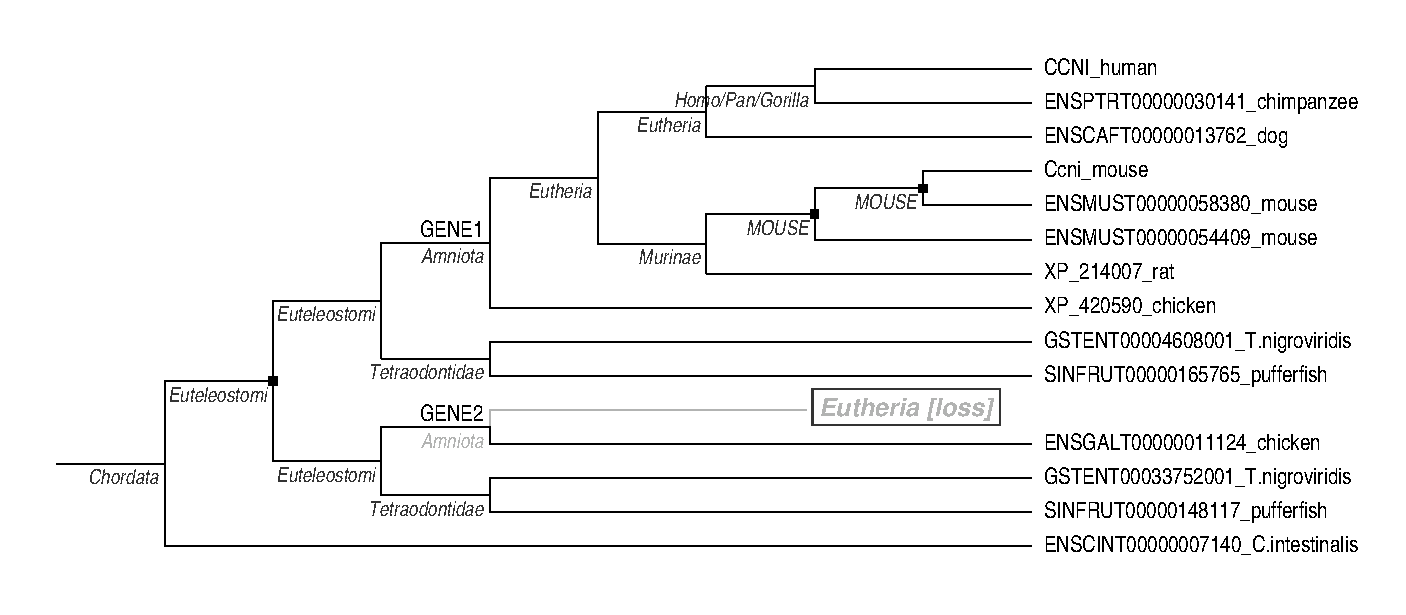
\includegraphics[width=\textwidth]{gtree}
\caption[Example of gene evolution]
{Example of gene evolution. A slant name beside an internal node
shows the ancestral species that contained the correponding ancestral gene. They are
actually $M^*(g)$ for each $g$ under parsimonious species map (Section~\ref{sec:specmap}). Duplications (the three bold nodes) and
loss (the gray boxed name) are inferred using methods that will be described in this chapter.}\label{fig:exa-dup-loss}
\end{center}
\end{figure}

The only way to infer duplications and losses is to compare the gene tree
to the species tree (Figure~\ref{fig:spectree}). This process is usually called \emph{tree reconciliation}\index{tree!tree reconciliation}
which was first suggested by Goodman~\cite{goodman79}, and implemented and improved by
many successors~\cite{page94,guigo96,eulenstein98}.
Recently, Zmasek and Eddy~\cite{zmasek01} have presented an elegant algorithm that greatly
simplifies duplication inference. Dufayard {\it et al.}~\cite{dufayard05} further developed
algorithms that could handle multifurcated species trees, though no detail is
provided. All these algorithms can be classified as parsimonious methods in
that the number of duplications and losses is minimized. A Bayesian method~\cite{arvestad03}
was also developed, which is claimed to be more effective in reducing missing duplication events.

In this chapter, we will introduce a generalized theory for duplication/loss inference,
and develop simple algorithms for such inference in the meantime. Our methods are based
on Zmasek and Eddy's work, but generalized in case of loss inference and
multifurcated species trees.

\section{Species Map}\label{sec:specmap}

To describe the inference of duplication/loss, it is necessary to bridge a gene tree
and a species tree. This bridge is called \emph{species map}\index{species map} that maps a gene, whether present or ancestral,
to the species that historically possessed the gene. When we know to which species a gene belonged,
we could pinpoint species evolution and gene evolution, reconstruct the history,
and smoothly infer the duplications and losses.

Mathematically, let $G$ be a gene tree, and $S$ a species trees, both \emph{rooted}.
Given $g\in V_E(G)$, a present gene, let $s_g\in V_E(S)$ be the species of gene $g$.
A map $M:V(G)\rightarrow V(S)$ is called a \emph{species map} if it satisfies the following
conditions for any $g\in V(G)$: (i) $M(g)=s_g$ if $g\in V_E(G)$, (ii) $s_{g'}\leq M(g)$ for all
$g'\in\omega_G(g)$ and (iii) $M(g)\leq M(g')$ if $g<g'$. Map $M$ embeds a species tree into
a gene tree and describes how the evolution of species shapes gene evolution.
In the following section, we will see that $M$ alone determines duplications and losses, and
thus how to choose $M$ is the key to duplication/loss inference.

\begin{figure}[!hb]
\begin{center}
\includegraphics{mpfig.4}\\*
\includegraphics{mpfig.5}
\end{center}
\caption[Example for illustrating species map]{Example for illustrating species map.
The top figure shows the parsimonious species map $M^*$ between species tree $S$ and gene tree $G$. Under
this map, each gene evolved normally. No duplication or loss occurred.
The bottom shows another species map $M'$ for the two trees. Under $M'$, at
least one historical duplication (at node $g'$) and two losses (showed in dashed branches)
occurred in this gene family. Note that in this example, branch length has no meanings.}\label{fig:specmap-exa}
\end{figure}

Given a specified gene tree and species tree, many maps will satisfy the two conditions.
Likelihood methods choose the one that maximizes the likelihood under certain statistical
model. This process is extremely time-consuming. In contrast, parsimony methods simply select the
the parsimonious species map\index{species map!parsimonious species map} $M^*$ that will lead to fewer duplications or losses in the end.
Without any proof here, we point out that $M^*$ can be simply constructed as:
\begin{equation}\label{equ:par-M}
M^*(g)=\lhlca(\{s_{g'}:g'\in\omega_G(g)\})
\end{equation}
Obviously $M^*$ is a species map, and in fact, $M^*(g)$ is the most recent
possible species to which $g$ belonged in history. Partly, this is also a reason why
$M^*$ is called a parsimonious map. Figure~\ref{fig:specmap-exa} gives an example of a parsimonious map and a common one.

\section{Duplication/Loss Inference (DLI)}

Ideally, a duplication can be observed if one species appears two or more times in
a gene tree. This is true if no loss occur. But when loss occur, this will overlook duplications.
We must recover the lost genes before we make such inference. For a binary species tree,
we can simply compare $M(g)$ and $M(\lhparent(g))$~\cite{zmasek01}, and infer $\lhparent(g)$ as a duplication
if $M(g)=M(\lhparent(g))$; for a multifurcated tree, however, this rule will
overestimate duplication events. As showed in Figure~\ref{fig:sigma}, both $g$ and
$g_p\equiv\lhparent(g)$ are mapped to {\it Eutheria}, but $g_p$ still represents speciation event, not
duplication. In order to generalize DLI (duplication/loss inference)\index{DLI, duplication/loss inference}
in case of a multifurcated species tree, it is helpful
to explicitly recover the species that are lost in gene trees.

\begin{figure}[!hb]
\begin{center}
\includegraphics{mpfig.3}
\end{center}
\caption[Example to explain $\sigma(g)$ set]{Example to explain $\sigma(g)$ set. In the left is a species tree $S$
with a multifurcated node; in the right is a gene tree $G$ with a loss. Node $g\in V(G)$
is mapped to $M^*(g)$ under the parsimonious map $M^*$, and $g_p$ mapped to $M^*(g_p)=M^*(g)$.
In this example,
$\sigma'(g)=\{{\it Human,Rat}\}$, $\sigma(g)=\{{\it Human,Mouse,Rat}\}$ and
$\omega_S(M^*(g))=\{{\it Human,Mouse,Rat,Dog}\}$. They are all different from one another:
$\sigma'(g)$ is smaller than $\sigma(g)$ because the mouse gene is lost,
while $\omega_S(M^*(g))$ is bigger because $M^*(g)$ is a trifurcation.}\label{fig:sigma}
\end{figure}

Given this fact, we introduce new notations:
\begin{equation}\label{equ:sigma0}
\sigma'(g)=\{s_{g'}:g'\in\omega_G(g)\}
\end{equation}
and
\begin{equation}\label{equ:sigma}
\sigma(g)=\sigma'(g)\cup\left\{s\in V_E(S):\mbox{$\exists s'\in\sigma'(g)$, $\lhlca(s,s')<M(g)$}\right\}
\end{equation}
While $\sigma'(g)$ only consists of present species that can be observed in the tree,
the second set in Equation~\ref{equ:sigma} also includes lost species in $G|_g$ subtree.
As a consequence, set $\sigma(g)$ consists of the species that should appear in $G|_g$ if no loss occurs in
this subtree.

Although the definition of $\sigma(g)$ looks complicated, it is irreplaceable.
This can be seen from the relation between the three sets $\sigma'(g)$, $\sigma(g)$ and $\omega_S(M(g))$:
$\sigma'(g)\subset\sigma(g)\subset\omega_S(M(g))$ where $\sigma'(g)=\sigma(g)$
stands if no loss occurs, while $\sigma(g)=\omega_S(M(g))$ if $M(g)$ is a binary node.
Figure~\ref{fig:sigma} also gives a concrete example where the three sets are different. As we will see in the following text,
$\sigma(g)$ plays a critical role on DLI.

\begin{figure}[!hb]
\begin{center}
\includegraphics[width=0.7\textwidth]{dli-exa}
\caption[Example of duplication/loss inference]
	{Example of duplication/loss inference. A slant name beside each internal node
	indicates the ancestral speices that contained the corresponding ancestral gene.
	Gray colour and slant leaves show the genes that cannot be observed nowadays due to loss events.
	In this gene tree, $\sigma(\mbox{\sf G1\_rat})=\{\mbox{\it Rat}\}$, $\sigma(\mbox{\sf G2\_chicken})=\{\mbox{\it Chicken}\}$,
	$\sigma(g_0)=\{\mbox{\it Huamn, Mouse, Rat, Chick}\}$ and $\sigma(g_1)=\{\mbox{\it Human, Mouse, Rat}\}$.
	Node $g_1$ is a speciation, and therefore $\lhloss(\mbox{\sf G1\_rat})=\lhloss'(\mbox{\sf G1\_rat})=\{\mbox{\it Mouse}\}$, while
	$g_0$ is a duplication and
	$\lhloss'(\mbox{\sf G2\_chicken})=\sigma(g_0)\setminus\sigma(\mbox{\sf G2\_chicken})=\{\mbox{\it Human, Mouse, Rat}\}$
	which makes $\lhloss(\mbox{\sf G2\_chicken})=\{\mbox{\it Eutheria}\}$.}\label{fig:dli-exa}
\end{center}
\end{figure}

\subsection{Inferring duplications and orthologs}

If $g\in V_E(G)$ is a duplication and no loss occurs in $G|_{g_1}$ and $G|_{g_2}$,
$\lhchild(g)=\{g_1,g_2\}$, we would expect to see $\sigma'(g_1)=\sigma'(g_2)$.
If losses occur, however, it is possible that $\sigma'(g_1)\cap\sigma'(g_2)=\emptyset$.
In this case, $\sigma(g)$ will play its role due to its inclusion of the lost species.
Formally, $g$ is a {\emph duplication}\index{duplication} (or duplication occurred at $g$) if
$\sigma(g_1)\cap\sigma(g_2)\neq\emptyset$, where $\lhchild(g)=\{g_1,g_2\}$. Figure~\ref{fig:dli-exa}
shows an example.

Orthologs are genes in different species that originate from a single gene in the last
common ancestor of these species~\cite{remm01}. Accordingly, in a gene tree, two present genes $g_1$ and
$g_2$ are said to be {\emph orthologs}\index{ortholog} if $\lhlca(g_1,g_2)$ is not a duplication.
This simple condition exactly capture the meaning of biological definition.

\subsection{Inferring losses}

We next seek to find a set $\lhloss(g)\subset V(S)$ that consists of species in which
gene losses occur when $g_p\equiv\lhparent(g)$ evolved into $g$. Note that
in this way, $\lhloss(g)$ will actually be localized at the branch between $g_p$ and $g$.
Thus the calculation at one node will not interfere with the calculation at another one, and
the total number of loss events in the tree $G$ is simply the sum of $|\lhloss(g)|$ of each node $g\in V(G)$.

As duplication and speciation represent different biological events, whether
$g_p$ is a duplication or not makes a little difference.
If $g_p$ is a duplication, subtree $G|_{g_p}$ and $G|_g$ should in theory consist of
same species. When this is violated, losses must happen and
$s\in\sigma(g_p)\setminus\sigma(g)$ covers all the species in which gene
losses occur. If $g_p$ is a speciation, besides the condition $s\in\sigma(g_p)\setminus\sigma(g)$,
a lost $s$ must appear only in $M(g_p)$'s subtree containing $M(g)$, or equivalently,
must satisfy $\lhlca(s,M(g))<M(g_p)$. We denote by $\lhloss'(g)$ the set of
present species that are lost in the gene tree\footnote{Given two sets $A$ and $B$,
$A\setminus B=\{a:\mbox{$a\in A$, and $a\notin B$}\}$.}:
\begin{equation}\label{equ:loss1}
\lhloss'(g)=\left\{\begin{array}{ll}
	\sigma(\lhparent(g))\setminus\sigma(g) & \mbox{if $\lhparent(g)$ is a duplication} \\
	\left\{s\in\sigma(\lhparent(g))\setminus\sigma(g):\lhlca(s,M(g))<M(\lhparent(g))\right\} & \mbox{otherwise}
	\end{array}\right.
\end{equation}
Set $\lhloss'(g)$ consists of present species that cannot be observed due to losses between $g$ and $g_p=\lhparent(g)$.
However, this is not good enough. A loss of ancestral species will cause the losses of
all the descendant present species. Based on parsimonious rule, we would like to count this as one loss event.
For this purpose, we define:
\begin{equation}\label{equ:loss2}
\lhloss(g)=\{s\in V(S):\omega_S(s)\subset\lhloss'(g),\omega_S(\lhparent(s))\not\subset\lhloss'(g)\}
\end{equation}
Set $\lhloss(g)$ avoids over-counting. It is actually the minimum set $A\subset V(S)$ satisfying $\omega_S(A)=\lhloss'(g)$.
Also take Figure~\ref{fig:exa-dup-loss} as an example. In this gene tree,
$\lhloss'(${\sf ENSGALT00000011124\_chicken}$)=\{\mathit{human,mouse,rat,dog}\}$ and
$\lhloss(${\sf ENSGALT00000011124\_chicken}$)=\{\mathit{Eutheria}\}$. {\it Eutheria} is just the species where the loss occured.
Figure~\ref{fig:dli-exa} gives another example.

\section{Duplication Function and Loss Function}\label{sec:dl-fun}
Both duplication function and loss function are defined on $V_I(G)$:
\begin{eqnarray}\label{equ:dl-fun}
D_G(g) &=& \left\{\begin{array}{ll}
	1 & \mbox{if $g$ is a duplication} \\
	0 & \mbox{otherwise}\end{array}\right. \\
L_G(g) &=& \sum_{g'\in\lhchild(g)}{|\lhloss(g')|}
\end{eqnarray}
Duplication function $D_G(g)$ measures whether $g$ is a duplication; loss function $L_G(g)$
counts losses when $g$ evolved into its children. Obviously, the total number of duplications and
losses in gene tree $G$ simply equal to $\sum D_G(g)$ and $\sum L_G(g)$ respectively.
Given a common species map $M$, the definitions of duplication and loss
functions must depend on the topology of the gene tree $G$, but if parsimonious species map
$M^*$ is applied, duplication and loss functions can be topology-independent.
This will be re-examined in Section~\ref{sec:re-dl-fun} when set representation is introduced.

\section{Towards Statistical Methods}

\begin{figure}[!hb]
\begin{center}
\includegraphics{mpfig.11}
\caption[Example showing the failure of parsimonious species map]
{Example showing the failure of parsimonious species map. Assume the
the true history of gene evolution included one duplication at {\it Eutheria} and two losses in
{\it Murinae} and {\it Human}. The human gene and the mouse gene are not orthologs. Arbitrarily applying the
parimonious species map $M^*$ will always miss these events and wrongly infer the two genes as orthologs.}\label{fig:bad-pars}
\end{center}
\end{figure}

In this section, we will come back to the selection of species map $M$ that
uniquely determines how the duplication and loss are inferred. Usually we only take
the parsimonious species map $M^*$ due to its simplicity, but unfortunately nature does not always
follow the parsimonious rule. In a multigene family
where duplications and losses tend to occur frequently, arbitrarily choosing $M^*$ might
underestimate the numbers and lead to more orthologs (Figure~\ref{fig:bad-pars}). More
sophisticated method that could possiblely select the species map other than $M^*$
should be applied this time. A Bayesian method has been introduced by
Arvestad {\it et al.}~\cite{arvestad03,arvestad04} and cleverly solve this problem.
We do not intend to present detailed description, which is far beyond the
scope of this thesis. We only add more remarks in comparison of parsimonious $M^*$ and
$M$ favoured by Bayesian method.

In Bayesian framework, the desired species map is the one that maximize the posterior
probability $\Pr\{M|G,S\}$, which can be calculated as:
\begin{eqnarray*}
\Pr\{M|G,S\}&=&\frac{\Pr\{M,G|S\}}{\Pr\{G|S\}}\\
	&=& \frac{1}{\Pr\{G|S\}}\cdot\int_{\mu}\int_{\lambda}\Pr\{M,G,\mu,\lambda|S\}\,d\mu\,d\lambda \\
	&=& \frac{1}{\Pr\{G|S\}}\cdot\int\!\!\!\int\Pr\{M,G|S,\mu,\lambda\}\Pr\{\mu,\lambda|S\}\,d\mu\,d\lambda \\
	&=& \frac{1}{\Pr\{G|S\}}\cdot\int\!\!\!\int\Pr\{M,G|S,\mu,\lambda\}p(\mu,\lambda|S)\,d\mu\,d\lambda \\
\end{eqnarray*}
where $\lambda$ is the birth rate, $\mu$ is the loss rate and
$p(\mu,\lambda|S)$ is the prior probability of $(\mu,\lambda)$ given a species tree $S$.
When no prior knowledge is available, we usually take bounded uniform distribution as what Arvestad {\it et al.}
has done. In this equation, $\Pr\{G|S\}$ is a constant given a specified $G$. Then all we should do
is to calculate $\Pr\{M,G|S,\mu,\lambda\}$. If we assume that when separated, whether by speciation or duplication,
genes evolved independently, $\Pr\{M,G|S,\mu,\lambda\}$ can be written as
the product of a series of independent factors\footnote{$M^{-\!1}:V(S)\rightarrow 2^{V(G)}$ can be regarded ass the reverse
of species map $M$.}:
\begin{equation}
\Pr\{M,G|S,\mu,\lambda\}=\prod_{s\in V(S)}\,\prod_{g\in M^{-\!1}(\lhparent(s))}q_G(g,s)
\end{equation}
where $q_G(g,s)$ is the probability of forming the observed gene tree when a single gene $g$ of $\lhparent(s)$ evolved into
its descendants of species $s$. Thus $\prod_{g\in M^{-\!1}(\lhparent(s))}q_G(g,s)$
represents the probability of forming the observed gene tree when species $\lhparent(s)$ evolved into $s$.
As to the calculation of $q_G(g,s)$, Arvestad {\it et al.} presents detailed descriptions base on previous works~\cite{nee94,yang97}.

%To demonstrate the advantage of Bayesian methods, Arvestad {\it et al.} showed two examples:
%the first was an MHC multigene family which contained many duplications
%and losses; the second example contained fewer duplications and losses, but they claimed that
%Bayesian method could give better support values. While the first example was appropriate, the second
%might be misleading. This can be accounted for by two reasons. First, the authors used
%MrBayes~\cite{huelsenbeck01} to generate, or reconstruct,  possible gene trees, and Bayesian method tends to yield `excessively high' support
%values~\cite{suzuki02,cummings03,simmons04}. And second, in their benchmark,
%both RIO~\cite{zmasek02} and OrthoStrapper~\cite{storm02} reconstruct resampled trees by Neighbour-joining that might be
%less accurate in comparison to likelihood method~\cite{kuhner94}. This will lead to lower support values, too.
%If RIO and OrthoStrapper had also inferred orthologs from gene trees reconstructed by MrBayes,
%they would probably have got similar support values.

Bayesian method establishes an elegant framework for tree reconciliation and also for
various complex analyses about gene evolution, including reconstructing species trees and gene trees
with the help of each other~\cite{arvestad04}.
However, Bayesian method might be faced with a few theoretical difficulties both in biological angle and
in mathematical angle. First of all, separated genes, either by duplication or speciation events, did not
evolve independently. Losses tended to occur after massive duplications. One-copy genes were also less likely to
be lost. These facts are not modeled in Bayesian framework at present.
Furthermore, Bayesian method has to work with
a prior distribution, which can improve the accuracy when correctly formed but may also induce bias when not carefully selected.
Unfortunately, bounded uniform distribution of $\lambda$ and $\mu$
is not appropriate. On one hand, from the known gene trees in TreeFam~\cite{li06},
birth rate $\lambda$ and death rate $\mu$ are centered around small values;
on the other hand, in order to deal with families with massive duplications
and losses where parsimony fails, bound values must be large enough. This produces the confliction.
Whereas the use of parsimonious map
never produces false duplications when the gene tree is correct, the use of Bayesian one will, and the use of such a uniform
distribution will further aggregate the problem because the higher probabilities
at larger $\lambda$ and $\mu$ tend to favour more duplications.
False duplications, which might cause more problems than
missing some, have to be evaluated before we apply Bayesian method in practice.

In most cases where $\mu$ and $\lambda$ are small, parsimonious species map $M^*$ is accurate enough.
Although in a complex gene family where duplications and losses frequently occurred it can be wrong, use of Bayesian method does not
give us more confidence when even the gene tree is questionable. Furthermore, under parsimonious
map duplication and loss functions also become topological independent.
These properties make $M^*$ particularly useful in Chapter~\ref{chap:merge}.

\chapter{Tree Merge} \label{chap:merge}

Phylogenetic trees are essential to various evolutionary studies.
Due to their irreplaceable positions, many algorithms were
developed to reconstruct phylogenetic trees, including distance-based
methods\index{tree building algorithm!distance-based},
parsimony methods~\cite{fitch71}\index{tree building algorithm!parsimonious},
max-likelihood algorithms~\cite{felsenstein81}\index{tree building algorithm!maximum-likelihood}
and the recent Bayesian methods~\cite{rannala96}\index{tree building algorithm!Bayesian}.
Whereas these algorithms establish the fundament of
the theory of tree reconstruction, they have to work with certain
evolutionary models in practice such as
JTT~\cite{jones92}\index{JTT},
WAG~\cite{whelan01}\index{WAG},
HKY~\cite{hasegawa85}\index{HKY},
GY94~\cite{goldman94}\index{GY94}, and many more.
Given the variety of algorithms and models, is there an ultimate solution
to tree reconstruction problems? Unfortunately, the answer is `no'.
One of the major causes is the evolutionary heterogeneity over time.
Shifts in site-specific evolutionary rates, which is usually termed
as `heterotachy'\index{heterotachy}, frequently occur~\cite{lopez02}.
A model best fit one lineage or time frame may lead to erroneous inference
in another. Although this fact has already been noticed in several previous
works~\cite{weiss03,susko02} and extensively studied in the case
of few sequences~\cite{kolaczkowski04,gadagkar05,spencer05,philippe05},
little was achieved in solving the problem practically. Evolutionists
still have to build trees with
various algorithms and models, and combine the results with prior
knowledges and personal experiences. But how on earth do they
assess different trees? Is there a way to achieve this automatically?
This chapter aims to answer these two questions.

\begin{figure}[!hb]
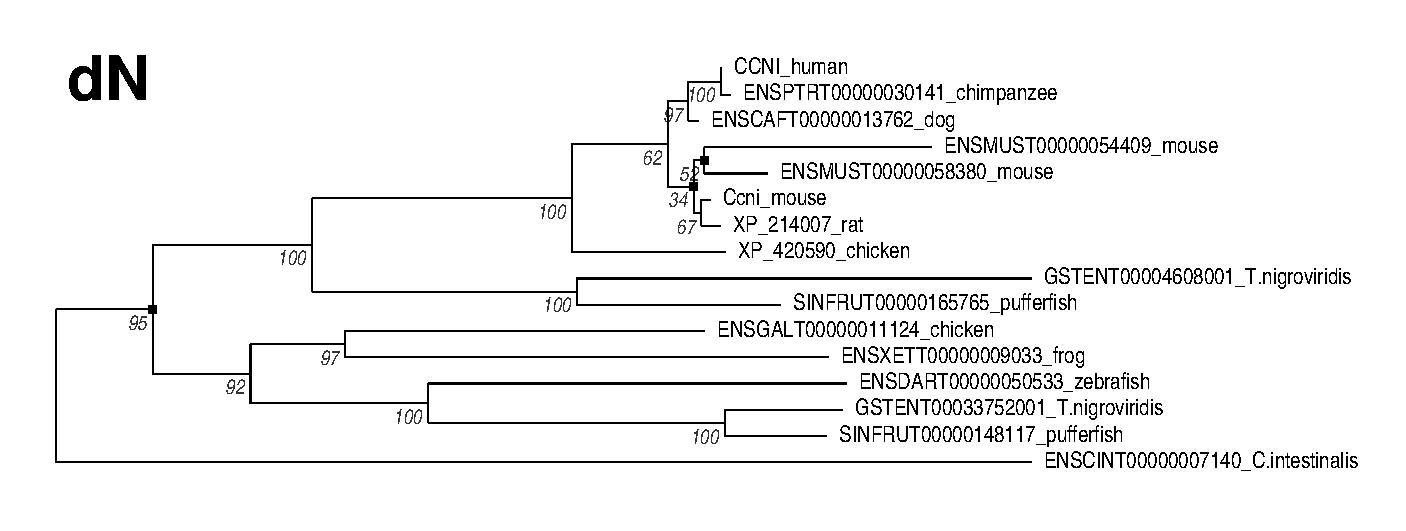
\includegraphics[width=\textwidth]{CCNI-dn}\\
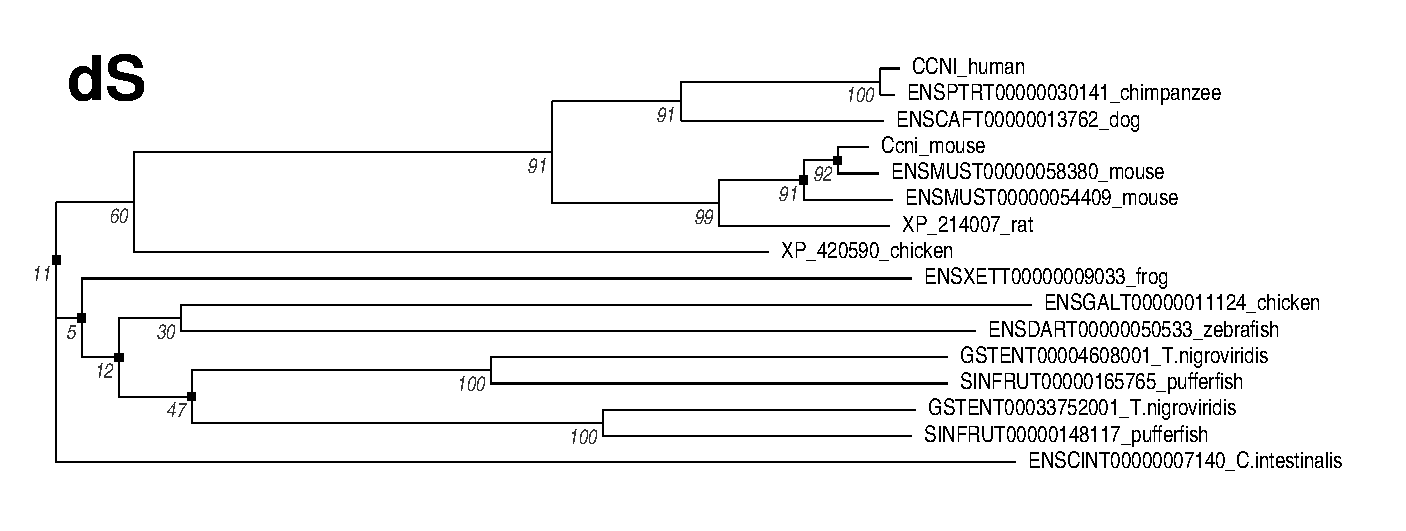
\includegraphics[width=\textwidth]{CCNI-ds}\\
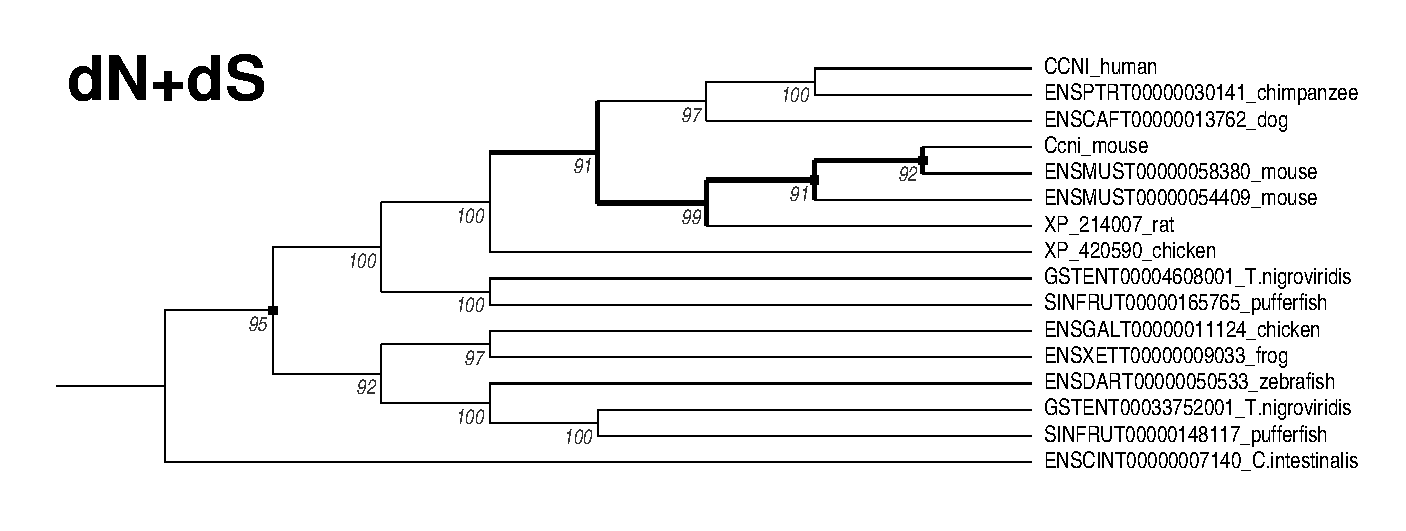
\includegraphics[width=\textwidth]{CCNI-dm}
\caption[Example of tree merge]{Example of tree merge. Non-synonymous tree {\bf dN}
	was merged with synonymous tree {\bf dS}, both reconstructed with neighbour-joining.
	Bold lines in the merged tree show the branches
	coming from {\bf dS}, while the rest from {\bf dN}. The resultant tree contains
	fewer losses and have higher bootstrapping support.	}\label{fig:mergeexam2}
\end{figure}

In order to understand how a tree can be evaluated by evolutionists,
let's first see an example. Figure~\ref{fig:mergeexam2} shows two trees reconstructed by neighbour-joining,
using synonymous distance ($d_s$) and non-synonymous
distance~\cite{nei86,li93,goldman94,yang00}\footnote{Nonsynonymous
distance ($d_n$) counts the number of nucleotide changes that contribute to
amino acid changes, while synonymous distance ($d_s$) counts the number that do not contribute to
amino acid changes.
Both kinds of distances can be only calculated in coding regions (CDS).
In theory, the synonymous distance $d_s$ tends to date the true evolutionary history more
precisely. Although selection for codon bias might occur, $d_s$ is generally less
influenced by heterogeneous selective pressure in different lineages~\cite{ayala99,baldauf03}.
However, if the two sequences are separated by a long evolutionary time, multiple
substitutions lead to saturation of $d_s$ and make it impossible to estimate $d_s$ accurately.
As a consequence, the deep branches of the $d_s$ tree are usually unreliable. Conversely, the
nonsynonymous distance $d_n$ is not saturated at long evolutionary time-frames and can
more effectively resolve the deep branches of the tree, but if the protein sequences are too similar,
too few non-synonymous changes will have accumulated to estimate $d_n$ accurately.
The lower branches of $d_n$ tree tend to be less accurate.} ($d_n$), respectively.
Even without any additional information, we can tell that the deeper branches
in $d_n$ tree and lower branches in $d_s$ tree are more likely to be correct.
This judgement is based on three rules: (i) reliable branches tend to
have higher bootstrapping support; (ii) synonymous trees are more effective
between close sequences, while nonsynonymous tree are better at deeper branches;
(iii) correct gene trees usually resemble the species tree.
If we can develop an algorithm that can account of these rules, it is possible
to automatically make a better tree by merging several trees built with different
methods. This is tree merge algorithm.

Tree merge is a process of choosing optimal
children between branches shared by candidate trees. As we want to shape the
algorithm in a precise and strict way, many abstract notations have to be used.
And therefore, we start this chapter by introducing the third type of representation of trees,
set representation. Then the tree merge problem is formally raised. After the description
and proof of the algorithm, we analyze the time complexity of this algorithm.
In the following chapter, the effectiveness of tree merge will be assessed together
with a lot of single-model algorithms.

\section{Set Representation of Trees}

Graph representation is more intuitive, but it is not convenient in comparing
rooted trees built from the same sequence set using different algorithms.
In graph language, identical trees are judged by comparing the
vertex sets and edge sets at the same time. But this is unnecessary. The edges or branches of a rooted
tree are naturally determined by the subset of leaves that are descendant from the lower node of the edge;
in turn, we can use a set of leaf subset to represent the topology of a rooted
tree~\footnote{Similarly, the topology of an unrooted tree can be represented as a set of
bipartitions of the leaf set}.
Thus, topological comparison can be reduced to set comparison, which is more
concise and straightforward.

\begin{figure}[!hb]
\begin{center}
\includegraphics{mpfig.10}
\caption[Example of set representation]
{Example of set representation. Set $\omega_G(g)$ is labeled at each internal node. The set representation
of $G$ is $\bar{G}=\{\{1\},\{2\},\{3\},\{4\},\{5\},\{2,3\},\{1,2,3\},\{1,2,3,4\},\{1,2,3,4,5\}\}$. Conversely,
when we get $\bar{G}$, we will also know the topology of $G$. Furthermore, if we let $\bar{g}=\{1,2,3\}$,
$\bar{G}|_{\bar{g}}=\{\{1\},\{2\},\{3\},\{2,3\},\{1,2,3\}\}$ is the set representation of $G|_g$.}\label{fig:example-set}
\end{center}
\end{figure}

Let $V$ be a leaf node set, and $\Sigma(V)=\{\mbox{$G$ is a rooted tree}:V_E(G)=V\}$ be the tree space in which each element
is a rooted tree whose external node set is $V$.
For any $G\in\Sigma(V)$, we can construct a set $\bar{G}\subset 2^V$~\footnote{Given a set $V$, $2^V=\{A:A\subset V\}$ is
the set of all the subsets of $V$ including $V$ itself and empty set $\emptyset$. $2^V$ is also called the $\sigma$-set of $V$.
Note that $\left|2^V\right|=2^{|V|}$ always stands. This is why it is written as $2^V$.}
using the $\omega_G$ map (Equation~\ref{equ:omega}) as follows:
\begin{equation}\label{equ:setrepre}
\bar{G}=\{\bar{g}\subset V:\bar{g}=\omega_G(g),g\in V(G)\}
\end{equation}
Obviously, $\bar{G_1}=\bar{G_2}$ only stands when the two trees $G_1$ and $G_2$ are topologically equivalent;
when $G_1$ differs $G_2$, $\bar{G_1}$ and $\bar{G_2}$ cannot be the same.
As a consequence, Equation~\ref{equ:setrepre} builds an one-to-one relation between
a set $\bar{G}$ and a graph $G$, and therefore $G$ can be represented by a set $\bar{G}$.
This is the set representation of a rooted tree.
When we know $\bar{G}$, we will always construct a tree $G$ under graph representation.
We also introduce:
\begin{equation}
\bar{G}|_{\bar{g}}=\{\bar{g}':\bar{g}'\in\bar{G}, \bar{g}'\subset\bar{g}\}
\end{equation}
Set $\bar{G}|_{\bar{g}}$ represents subtree $G|_g$. Figure~\ref{fig:example-set} shows an example.

Throughout this chapter, notations like $\bar{G}$ and $\bar{g}$ are always under the set representation.

\section{Set Forms of Duplication and Loss Functions}\label{sec:re-dl-fun}

In Section~\ref{sec:dl-fun}, the duplication and loss functions are defined as (Equation~\ref{equ:dl-fun}):
\begin{eqnarray}\label{equ:dl-fun-set}
D_G(g) &=& \left\{\begin{array}{ll}
    1 & \mbox{if $g$ is a duplication} \\
    0 & \mbox{otherwise}\end{array}\right. \\
L_G(g) &=& \sum_{g'\in\lhchild(g)}{|\lhloss(g')|}
\end{eqnarray}
The two functions defined in this way are dependent on the topology of the gene tree $G$.
As a matter of fact, if the parsimonious species map $M^*$ is applied to infer duplications and losses, the two functions
can be defined in a way independent of $G$. Let's re-examine the deduction of duplication and loss
under set representation.

In the following text, we always let $\bar{g}$, $\bar{g}_1$ and $\bar{g}_2$
be a subset of $V_E(G)$. From Equation~\ref{equ:par-M} and~\ref{equ:sigma}, we define:
\begin{eqnarray}
\sigma'(\bar{g}) &=& \{s_{g'}:g'\in \bar{g}\} \\
M^*(\bar{g}) &=& \lhlca(\sigma'(g)) \\
\sigma(\bar{g}) &=& \sigma'(g)\cup\left\{s\in V_E(S):\mbox{$\exists s'\in\sigma'(g)$, $\lhlca(s,s')<M^*(\bar{g})$}\right\}
\end{eqnarray}
Thus the parsimonious duplication function is:
\begin{equation}
D^*(\bar{g}_1,\bar{g}_2)=D^*(\bar{g}_2,\bar{g}_1)=\left\{\begin{array}{ll}
	1 & \mbox{if $\sigma(\bar{g}_1)\cap\sigma(\bar{g}_2)\not=\emptyset$;} \\
	0 & \mbox{otherwise.}\end{array}\right.
\end{equation}
Parsimonious loss function can be defined in a similar way:
\begin{equation}
L^*(\bar{g}_1,\bar{g}_2)=L^*(\bar{g}_2,\bar{g}_1)=|\lhloss^*(\bar{g}_1,\bar{g}_2)|+|\lhloss^*(\bar{g}_2,\bar{g}_1)|
\end{equation}
where
\begin{equation}
\lhloss'^*(\bar{g}_1,\bar{g}_2) = \left\{\begin{array}{ll}
	\sigma(\bar{g}_1\cup\bar{g}_2)\setminus\sigma(\bar{g}_1) & \mbox{if $D^*(\bar{g}_1,\bar{g}_2)=1$} \\
	\{s\in\sigma(\bar{g}_1\cup\bar{g}_2)\setminus\sigma(\bar{g}_1):\lhlca(s,M^*(\bar{g}_1))<M^*(\bar{g}_1\cup\bar{g}_2)\} & \mbox{otherwise}
\end{array}\right.
\end{equation}
\begin{equation}
\lhloss^*(\bar{g}_1,\bar{g}_2) = \{s\in V(S):\omega_S(s)\subset\lhloss'(\bar{g}_1,\bar{g}_2),\omega_S(\lhparent(s))\not\subset\lhloss'(\bar{g}_1,\bar{g}_2)\}
\end{equation}
They correspond to Equation~\ref{equ:loss1} and~\ref{equ:loss2}.
Now, parsimonious duplication and loss functions can be calculated given two set of leaves.
Such calculation is topology-independent in the sense that the topologies on the two sets
will not affect the calculation process. This property is particularly useful
in constructing the objective function for tree merge algorithm~\ref{sec:merge-obj-fun}.

\section{Tree Merge}

\subsection{Tree merge problem}

Given a set of \emph{binary rooted} trees $\Phi=\{\bar{G}_1,\bar{G}_2,\ldots,\bar{G}_n\}$, define a permitted branch set:
\begin{equation}
\mathcal{G}(\Phi)=\bigcup_{\bar{G}'\in\Phi} \bar{G'}
\end{equation}
Let $\Omega(\mathcal{G})$ be the set of binary rooted tree $\bar{G}$ that satisfies $\bar{G}\subset\mathcal{G}$.
Being a subset of $\Sigma(V)$, $\Omega(\mathcal{G})$
is the tree space spanned by $\bar{G}_1,\bar{G}_2,\ldots,\bar{G}_n$.
It is also useful to define a permitted branch set $\mathcal{G}|_{\bar{g}}$ that
is restricted to a node $\bar{g}$:
\begin{equation}
\mathcal{G}|_{\bar{g}} = \bigcup_{\bar{G}'\in\Phi} \bar{G}'|_{\bar{g}}
\end{equation}
Then $\Omega(\mathcal{G}|_{\bar{g}})$ is the tree space spanned by $\bar{G}_1|_{\bar{g}},\bar{G}_2|_{\bar{g}},\ldots,
\bar{G}_n|_{\bar{g}}$.

Let $F$ be a function defined on $\Sigma(V)$. The \emph{general tree merge problem}
\index{tree merge problem!general tree merge problem} is to find a \emph{binary rooted} tree
$\bar{G}\in\Omega(\mathcal{G})$ that optimizes $F(\cdot)$. For common $F$, the only solution is to
enumerate every tree in $\Omega$ and then search for the optimum one. But for
a class of special objective functions, the exhaustive search can be replaced by a simple precise
algorithm. In this thesis, we only consider functions that take the form:
\begin{equation}\label{equ:independent}
F(\bar{G})=\sum_{\bar{g}\in \bar{G}}f(\lhchild(\bar{g}))=\sum_{\bar{g}\in \bar{G}}f(\bar{g}_1,\bar{g}_2)
\end{equation}
Such an $F(\bar{G})$ has two critical properties. First, it is additive, and second,
function $f$ is defined on $2^V\times 2^V$, which means that the calculation of $f(\lhchild(\bar{g}))$ is
only dependent on the elements in $\bar{g}$'s children set but independent of the topologies of
$\bar{g}$'s children. As we will see in the following section,
these two properties, especially the second one, guarantee that the optimum tree can be
found in $O(|\Phi|\cdot|V|^2)$ time.
The (special) \emph{tree merge problem}\index{tree merge problem} is to find the optimal \emph{binary rooted} tree
in $\Omega(\mathcal{G})$ when $F(\bar{G})$ follows Equation~\ref{equ:independent}.

\subsection{Constructing objective functions}\label{sec:merge-obj-fun}

According to Equation~\ref{equ:independent}, the effectiveness of tree merge algorithm
totally relies on function $f$. Before detailed algorithm is described, we should make
sure that $f$ is present and biologically reasonable.

Based on the discussion in Section~\ref{sec:re-dl-fun}, $f$ can be defined as:
\begin{equation}\label{equ:f-obj}
f(\bar{g}_1,\bar{g}_2)=f(\bar{g}_2,\bar{g}_1)=\alpha D^*(\bar{g}_1,\bar{g}_2)
	+\beta L^*(\bar{g}_1,\bar{g}_2)-\gamma B^*(\bar{g}_1,\bar{g}_2)
\end{equation}
where $\alpha,\beta,\gamma>0$, $D^*(\bar{g}_1,\bar{g}_2)$ and $L^*(\bar{g}_1,\bar{g}_2)$ are
the duplication and losses functions, respectively, and $B^*(\bar{g}_1,\bar{g}_2)$ denotes
the highest bootstrapping supports among all trees containing $\{\bar{g}_1,\bar{g}_2\}$.
Note that the star in in $D^*$ and $L^*$ indicates the parsimonious species map
$M^*$ is used in DLI inference. These two functions measure the similarity between
a gene tree and the species tree. The smaller, the better.
As to $B^*(\bar{g}_1,\bar{g}_2)$, another possible
definition is also available, which will be discussed in the end of this chapter.
%However, when the majority of candidates
%are built from similar algorithms, such a $B^*$ will favour
%them because similar algorithms tend to result in similar topologies.
%And therefore the previous definition is more appropriate.
In addition, if we know
that certain algorithm is good at particular branches, we can deliberately
raise the bootstrapping supports. Consequently, all the three rules addressed in
the introduction section of this chapter have been considered.

\subsection{Tree merge algorithm}

The basic idea of tree merge algorithm resembles that of dynamic programming. It reduces
exhaustive search to the calculation of a function $F^*(\bar{g})$ for each $\bar{g}\in\mathcal{G}$.
$F^*$ is defined as:
\begin{equation}\label{equ:F-star}
F^*(\bar{g}) = \min_{\bar{G}|_{\bar{g}}\in\Omega(\mathcal{G}|_{\bar{g}})} F(\bar{G}|_{g})
\end{equation}
Obviously, $F^*(V) = \min F(\bar{G})$ always stands. Thus searching optimal tree $\bar{G}$
is equivalent to calculating $F^*(V)$. When $F(\cdot)$ follows Equation~\ref{equ:independent},
$F^*(V)$ can be calculated recursively. To achieve this goal, we need to construct
the set of permitted children pairs given a node $\bar{g}$:
\begin{equation}\label{equ:C-set}
\mathcal{C}(\bar{g}) = \left\{\{\bar{g}_1,\bar{g}_2\}:\mbox{$\bar{g}_1,\bar{g}_2\in\mathcal{G}$, $\bar{g}_1\cap\bar{g}_2=\emptyset$ and $\bar{g}_1\cup\bar{g}_2=\bar{g}$}\right\}
\end{equation}
Set $\mathcal{C}(\bar{g})$ consists of $\bar{g}$'s candidate children set. That is,
each element $\{\bar{g}_1,\bar{g}_2\}\in\mathcal{C}(\bar{g})$ can be $\bar{g}$'s children set. Then,
\begin{eqnarray*}
&&F^*(\bar{g})\\
&=& \min_{\bar{G}|_{\bar{g}}\in\Omega(\mathcal{G}|_{\bar{g}})} F(\bar{G}|_{g})\\
&=& \min_{\bar{G}|_{\bar{g}}\in\Omega(\mathcal{G}|_{\bar{g}})}\sum_{\bar{g}'\in \bar{G}|_{\bar{g}}}f(\lhchild(\bar{g}')) \\
&=& \min_{\{\bar{g}_1,\bar{g}_2\}\in\mathcal{C}(\bar{g})}\left\{
	\min_{\bar{G}|_{\bar{g}_1}\in\Omega(\mathcal{G}|_{\bar{g}_1})}\sum_{\bar{g}'_1\in \bar{G}|_{\bar{g}_1}}f(\lhchild(\bar{g}'_1))
	+ f(\bar{g}_1,\bar{g}_2)
	+ \min_{\bar{G}|_{\bar{g}_2}\in\Omega(\mathcal{G}|_{\bar{g}_2})}\sum_{\bar{g}'_2\in \bar{G}|_{\bar{g}_2}}f(\lhchild(\bar{g}'_2))\right\}
\end{eqnarray*}
From Equation~\ref{equ:F-star} and~\ref{equ:independent}, we know that:
\begin{equation}\label{equ:cal-F-star}
F^*(\bar{g}) = \min_{\{\bar{g}_1,\bar{g}_2\}\in\mathcal{C}(\bar{g})}\left\{F^*(\bar{g}_1)+f(\bar{g}_1,\bar{g}_2)+F^*(\bar{g}_2)\right\}
\end{equation}
Thus $F^*(V)$ can be calculated recursively.

\begin{table}[!hb]
\begin{center}
\begin{tabular}{|l|}
\hline
{\bf Function:}\\
\lhspace{\sc TreeMerge}$(V,\bar{G}_1,\bar{G}_2,\ldots,\bar{G}_n)$\\
{\bf Input:} \\
\lhspace$n$ gene trees $\bar{G}_1,\bar{G}_2,\ldots,\bar{G}_n\in\Sigma(V)$; \\
{\bf Output:} \\
\lhspace Tree $\bar{G}^*$ by merging $\bar{G}_1,\bar{G}_2,\ldots,\bar{G}_n$\\
{\bf Procedures:} \\
\lhspace$\mathcal{G}\leftarrow\emptyset$ \\
\lhspace$\mathcal{C}\leftarrow\emptyset$ \\
\lhspace{\sc ConstructG}$(\bar{G}_1,\ldots,\bar{G}_n)$ \\
\lhspace\lhspace{\bf for} $i = 1$ {\bf to} $n$ {\bf do} \\
\lhspace\lhspace\lhspace{\bf for} each $\bar{g}\in \bar{G}_i$ {\bf do} \\
\lhspace\lhspace\lhspace\lhspace$\mathcal{G}\leftarrow\mathcal{G}\cup\{\bar{g}\}$ \\
\lhspace\lhspace\lhspace\lhspace$\mathcal{C}(\bar{g})\leftarrow\mathcal{C}(\bar{g})\cup\{\lhchild(\bar{g})\}$ \\
\\
\lhspace$selected\gets\emptyset$\\
\lhspace{\sc OptimizeF}$(\bar{g})$ \\
\lhspace\lhspace{\bf if} $F^*(\bar{g})$ has been calculated {\bf then} \\
\lhspace\lhspace\lhspace{\bf return} $F^*(\bar{g})$ \\
\lhspace\lhspace$min\leftarrow\infty$ \\
\lhspace\lhspace{\bf for} each $\{\bar{g}_1,\bar{g}_2\}\in\mathcal{C}(\bar{g})$ {\bf do} \\
\lhspace\lhspace\lhspace$score\gets\mbox{{\sc OptimizeF}}(\bar{g}_1)+f(\bar{g}_1,\bar{g}_2)+\mbox{{\sc OptimizeF}}(\bar{g}_2)$\\
\lhspace\lhspace\lhspace{\bf if} $min>score$ {\bf then}\\
\lhspace\lhspace\lhspace\lhspace$min\gets score$\\
\lhspace\lhspace\lhspace\lhspace$minpair\gets \{\bar{g}_1,\bar{g}_2\}$\\
\lhspace\lhspace$F^*(\bar{g})\gets min$ \\
\lhspace\lhspace$selected(\bar{g})\gets minpair$ \\
\\
\lhspace{\sc BuildTree}$(\bar{g})$ \\
\lhspace\lhspace{\bf if} $selected(\bar{g})=\emptyset$ {\bf then}\\
\lhspace\lhspace\lhspace{\bf return} $\{\bar{g}\}$\\
\lhspace\lhspace$\{\bar{g}_1,\bar{g}_2\}\gets selected(\bar{g})$\\
\lhspace\lhspace{\bf return} $\mbox{\sc BuildTree}(\bar{g}_1)\cup\{\bar{g}\}\cup\mbox{\sc BuildTree}(\bar{g}_2)$\\
\\
\lhspace{\sc TreeMerge}$(V,\bar{G}_1,\bar{G}_2,\ldots,\bar{G}_n)$\\
\lhspace\lhspace{\sc ConstructG}$(\bar{G}_1,\ldots,\bar{G}_n)$\\
\lhspace\lhspace{\bf for} each $v\in V$ {\bf do}\\
\lhspace\lhspace\lhspace$F^*(\{v\})\gets 0$\\
\lhspace\lhspace{\sc OptimizeF}$(V)$\\
\lhspace\lhspace{\bf return} {\sc BuildTree}$(V)$\\
\hline
\end{tabular}
\caption[Tree merge algorithm]
{Tree merge algorithm. Procedure {\sc ConstructG} constructs $\mathcal{G}$ and $\mathcal{C}(\bar{g})$;
{\sc OptimizeF} recursively calculates $F^*(\bar{g})$ and stores optimum children
in $selected$, from which {\sc BuildTree} builds the merge tree. {\sc BuildTree}
generates a tree in set presentation. It can also be easily adapted to generate a tree
$G^*=(V(G^*),E(G^*))$ in graph presentation.}~\label{tab:merge}
\end{center}
\end{table}

\begin{figure}[!hb]
\begin{center}
\includegraphics{mpfig.7}
\caption[Example of tree merge algorithm]{Example of tree merge algorithm. Tree $G_1$ and $G_2$ are
merged into $G^*$. Bold nodes show the duplications and the number beside a branch is
the number of losses occuring at that branch. For example, $|\lhloss(\{mou_1\},\bar{g}_3)|=|\{{\it Rat}\}|=1$
and $|\lhloss(\bar{g}_1^c,\bar{g}_6)|=|\{{\it Human, Chicken}\}|=2$.}\label{fig:merge-exa}
\end{center}
\end{figure}

The two equations, \ref{equ:C-set} and \ref{equ:cal-F-star}, established the basis of tree merge algorithm. Table~\ref{tab:merge}
presents more details. In practical implementation, hash technique should be applied
to judge whether $\bar{g}$ has been inserted to $\mathcal{G}$. If the hash function
is perfect, only $O(|V|)$ time is needed to locate and insert a set to $\mathcal{G}$.
This will greatly accelerate the algorithm.

Hash technique makes tree merge very efficient. In procedure {\sc ConstructG}, all the hash values can be
calculated in $O(n\cdot|V|(|V|-1))$. The following $n\cdot(|V|-1)$ times of set comparisons and insertions
take $O(n\cdot|V|^2)$ time at most. Procedure
{\sc OptimizeF} traverses all possible $\bar{g}\in\mathcal{G}$ and $\bar{g}$'s bipartition
$\bar{g}=\bar{g}_1\cup\bar{g}_2$. The time complexity in this part is also $O(n\cdot|V|^2)$.
Both {\sc BuildTree} and {\sc TreeMerge} can be achieved in $O(|V|)$. Consequently, the time complexity
of tree merge is $O(n\cdot|V|^2)$.

Figure~\ref{fig:merge-exa} gives an example of tree merge process.
In this example, $\mathcal{G}=\{\{hum\},\{mou_1\},\{mou_2\},\{rat\},\{chi\},\bar{g}^c_1,
\bar{g}^c_2,\bar{g}_3,\bar{g}_4,\bar{g}_5,\bar{g}_6\}$,
$\mathcal{C}(\bar{g}^c_1)=\left\{\{\bar{g}_3,\{mou_2\}\},\{\{rat\},\bar{g}_5\}\right\}$
and $\mathcal{C}(\bar{g}^c_2)=\left\{\{\bar{g}_4,\{chi\}\},\{\bar{g}^c_1,\bar{g}_6\}\right\}$.
Only $\mathcal{C}(\bar{g}^c_1)$ and $\mathcal{C}(\bar{g}^c_2)$ consist of more than one node pairs. Other $\mathcal{C}(\cdot)$ just
has one element. If we let $\alpha=\beta=1$ and $\gamma=0$ in Euqation~\ref{equ:f-obj},
we know that $f(\bar{g}_3,\{mou_2\})=1+1=2$, $f(\{rat\},\bar{g}_5)=0$, $F^*(\bar{g}_5)=1$ and $F^*(\bar{g}_3)=0$. Thus
$F^*(\bar{g}^c_1)=\min\{0+2+0,0+0+1\}=1$. The children pair $\{\{rat\},\bar{g}_5\}$ is preferable.
Similarly, as $f(\bar{g}_4,\{chi\})=0$, $f(\bar{g}^c_1,\bar{g}_6)=3$, $F^*(\bar{g}_4)=1+0+0=1$
and $F^*(\bar{g}_6)=1$, $F^*(\bar{g}^c_2)=\min\{1+0+0,1+3+1\}=1$.
The children pair $\{\bar{g}_4,\{chi\}\}$ is preferred. Consequently,
$\bar{G}^*=\{\{hum\},\{mou_1\},\{mou_2\},\{rat\},\{chi\},\bar{g}_1^c,\bar{g}_2^c,\bar{g}_4\}$ gives the final tree
and $F(G^*)=F^*(\bar{g}^c_2)=1$.

\section{Discussions}
Tree merge is able to capture the thinking of evolutionists. Although not
a tree-building algorithm by itself, tree merge can combine the advantages of
different tree-building algorithms and models, and automatically choose suitable
methods in different lineages. It is most useful when candidate trees
can compensate for the deficiency of one another. However,
just as evolutionists cannot reconstruct correct trees
without reasonable candidate trees, tree merge is less useful or even wrong
if artefact candidates are provided. Sometimes a human being can detect the artefacts
and make a tree outside $\Omega$ tree space, but tree merge cannot achieve.
This is the theoretical limitation. Furthermore, the performance of tree merge is
determined by the objective function. An evolutionary history that breaks
the optimization process will fail tree merge, either.
When using tree merge algorithm, we should pay attention to these points.

Tree merge algorithm can also be considered as an alternative algorithm to make
a consensus tree~\cite{margush81} from a set of resampled trees. All we need is to modify the definition of $B^*(\bar{g}_1,\bar{g}_2)$
in Equation~\ref{equ:f-obj}. Assume we have $n$ resampled binary rooted gene trees $\Phi=\{\bar{G}_1,\bar{G}_2,\ldots,\bar{G}_n\}$.
Given $\bar{g}_1,\bar{g}_2\in\mathcal{G}(\Phi)$, we can define $B^*(\bar{g}_1,\bar{g}_2)$ as the number of times when
$\{\bar{g}_1\cup\bar{g}_2\}\subset\bar{G}_i$, $i=1,\ldots,n$\footnote{$B^*$
can also be defined in other similar, but different, ways.}. In this way,
$B^*(\bar{g}_1,\bar{g}_2)$ is the bootstrapping supports for a branch $\{\bar{g}_1,\bar{g}_2\}$.
And if we set $\alpha=\beta=0$, tree merge process is actually the same as that of making a consensus tree from a set of
binary rooted trees. In conclusion, when $B^*$ is defined as above, tree merge extends (rooted) consensus
tree algorithms by incorporating species evolution, and may help to improve the quality of the consensus tree.

Tree merge is designed to work with a binary rooted gene tree where the phylogeny
of species is clear. How to root a tree was discussed in~\ref{chap:buildtree}.
In principle, it is also possible to extend the algorithm in case of unrooted trees,
but most of concepts in this chapter should be modified accordingly.
Resolving a multifurcated tree is also tactable. Durand {\it et al.}~\cite{durand06} implies
an algorithm that may be adapted to resolve polytomies by minimizing duplications and losses.
In contrast, the requirement of species phylogeny is critical. To our experience, no other criterion that
satisfies Equation~\ref{equ:independent} can be as effective as this standard.

\chapter{Evaluation of Tree Building Methods}\label{chap:benchmark}

Whereas the variety of tree-building algorithms give evolutionists the opportunities
to choose the one that best fits the data, the disagreements between these
algorithms also confuse researchers at times. Given a set of sequences, it is not
always clear what method is most effective on a certain condition. In case
of one or a few sets of sequences, it is possible to manually curate the resultant trees.
But in the case of large-scale analysis for hundreds of gene families, such a process is formidable.
Even if massive manual curation can be achieved in the long run, which is major goal of TreeFam~\cite{li06},
guild-lines on successful tree-building are definitely beneficial to reduce manual work and
meanwhile avoid artifacts in curation.

A number of studies have been done to investigate the performance of these algorithms.
Based on the characteristics of the data sets in use, these studies can be classified into
three types: theoretical analysis on 4- or 5-leaf trees~\cite{gaut95,huelsenbeck95,yang96}, computational simulation
on large data sets~\cite{kuhner94,hall05,hollich05}, and real data from experimental manipulations~\cite{hillis92,hillis94,bull97}.
Although these studies did provide invaluable information on evaluating different algorithms, they
may still suffer a number of problems respectively: theoretical analysis can only
be applied to very small trees; computational simulation has to work with proposed evolutionary models or processes;
experiment-manipulated data are relatively small and usually developed on a special condition
that may deviate from real evolutionary processes. The most realistic evaluation is expected
to be done with large-scale data that are formed in true evolutionary history, which,
unfortunately, is unknown to us. Is there a way out?

In this chapter, we try to present a novel evaluation on various tree-building algorithms.
It differs from previous studies on two aspects: the use of large-scale curated
real data from TreeFam, and the use of model-independent indication:
duplications and losses tend to be minimized. Limited to the potential curation errors in real data and
the possibility that true evolution might favour more duplications and losses in some cases,
it is still too early to make a final conclusion about what algorithm is superior.
We only intend to show some data that will help evolutionists
to choose the most appropriate algorithms in practical use.

\section{Evaluated Algorithms and Evolutionary models}

Three classical algorithms,
distance-based method\index{tree building algorithm!distance-based},
parsimony~\cite{fitch71}\index{tree building algorithm!parsimonious} and
ML (Maximum Likelihood)~\cite{felsenstein81} method\index{tree building algorithm!maximum-likelihood},
were tested at both nucleotide level and amino acid level. Two types of merged trees were also
included. Table~\ref{tab:eval-algo} shows the 17 types of trees
used in this benchmark. More details will be explained as follows.

Distance-based method is actually the name of a group of algorithms including
Fitch-Margoliash~\cite{fitch67}\index{Fitch-Margoliash},
ME (Minimum Evolution)~\cite{rzhetsky93}\index{ME, minimum evolution},
UPGMA~\cite{sokal58}\index{UPGMA},
NJ (Neighbour-Joining)~\cite{saitou87}\index{NJ, neighbour-joining}
and several alternatives to standard NJ algorithms. In this benchmark, only standard NJ and ME
algorithms were tested in consideration of their popularity and accuracy.
NJ tree was built by NJTREE\index{NJTREE} and ME tree by FastME in GME framework~\cite{desper04}.
Distance matrix was calculated by TREE-PUZZLE~\cite{schmidt02}\index{TREE-PUZZLE}.
For nucleotide alignment, HKY~\cite{hasegawa85} model\index{HKY} was applied with
transition/transversion ratio\footnote{Transitions denote the nucleotide changes between purines
(A$\leftrightarrow$G) or between pyrimidines (C$\leftrightarrow$T),
while other types of nucleotide changes are all transversions. Biologically, transitions occur more frequently
than transversions, and therefore they are modeled differently.} estimated from data; for amino acids alignment,
WAG~\cite{whelan01}\index{WAG}
was used. In both cases, we fixed the shape factor $\alpha=1.0$ of $\Gamma$ distribution
which was approximated by 4 discrete substitution rate categories~\cite{yang94}. Alignment gaps
were regarded as missing data\footnote{Likelihood methods are capable of treating gaps as missing data
while calculating the distances. This is more robust.} in TREE-PUZZLE. As TreeFam-1.x trees were built from NJ with
p-distance\index{p-distance}\footnote{P-distance is also called mismatch distance. It actually equals to
the percent mismatches in the matched regions of two sequences.},
a distance without correction for in-site multiple substitutions\footnote{In-site multiple
substitutions denote multiple substitutions occurring at the same site.
For example, at a certain site nucleotide Adenine (A) was changed into nucleotide Guanine (G) 100 million years ago,
but 50 million years ago, the Guanine (G) was changed back to Adenine (A). Then two substitutions should be
counted even if no substitution is observed nowadays. A sophisticated evolutionary model can estimate how
often this is the case. But when sequences are too diverged, the variance of such estimation will be very large,
and therefore less accurate.}, this simplest model was also tested this time.

Parsimonious trees were reconstructed by {\bf dnapars} and {\bf protpars}, respectively.
Both programs are included in PHYLIP package~\cite{felsenstein89}\index{PHYLIP}. Tree merge
was applied if several optimal trees were given by the programs.
In our test, {\bf protpars} only presents binary trees, but {\bf dnapars} may build
multifurcated trees. As both duplication/loss inference and tree merge algorithm only work with binary trees,
some trees built by {\tt dnapars} could not be processed.

PHYML~\cite{guindon03}\index{PHYML} built ML trees. Parameters of evolutionary models are identical
to the ones used in TREE-PUZZLE. That is, HKY for nucleotide and WAG for amino acids;
substitution rates were divided into 4 discrete categories that approximated a $\Gamma$ distribution
with $\alpha=1.0$. Two or one categories were also evaluated to confirm the role
of $\Gamma$ distribution.
It seems that PHYML and TREE-PUZZLE implemented models in slightly different ways.
This can be observed when they were used to optimize branch length
given a specified tree. When we assume substitutions occur uniformly across sites (one category),
PHYML and TREE-PUZZLE can always achieve almost the same results. However,
when more than one categories are applied, their results differ more or less.
But as PHYML is unable to give a distance matrix while TREE-PUZZLE cannot
make standard ML trees, this minor inconsistency has to be tolerated.

Two trees generated by tree merge algorithm were also assessed. The first one was built by merging
a synonymous tree and a non-synonymous tree; the second by merging two ML trees and
also synonymous and non-synonymous trees. As to the objective function $f$ (Equation~\ref{equ:f-obj}),
we set $\alpha=100000$, $\beta=1000$ and $\gamma=1$. Bootstrapping values $B$ was
scaled between 0 and 100. This setting always prefers less duplications, and less losses only if
duplications are the same. Bootstrap only works when both $D^*$ and $L^*$
are identical. Due to efficiency issue, bootstrapping was not applied to
ML trees. We arbitrarily set bootstrapping support as 80 at each internal branches (branches that do not connect leaves)
given the fact that ML trees tend to be more reliable~\cite{kuhner94}.
Here, bootstrapping values are least favoured because a single tree-building algorithm
might also have high bootstrapping supports at wrong branches. Duplications are better
than losses because in evolution, duplications occur more rarely while losses more frequently, especially
following a duplication event.

\begin{table}
\begin{center}
\begin{tabular}{|l|l|}
\hline
Name & Method \\
\hline
{\tt CUR} & Curated trees from TreeFam \\
\hline
{\tt NJ-NT-HKY4} & Neighbour-Joining, HKY model, $C=4$, $\alpha=1.0$, $\kappa$ estimated \\
{\tt NJ-AA-WAG4} & Neighbour-Joining, WAG model, $C=4$, $\alpha=1.0$ \\
{\tt NJ-NT-dN} & NJ, non-synonymous distance, no correction for multi-substitutions \\
{\tt NJ-NT-dS} & NJ, synonymous distance, no correction for multi-substitutions \\
{\tt NJ-AA-MM} & NJ, p-distance (or mismatch) distance, no correction \\
{\tt NJ-AA-Kmr} & NJ, with Kimura correction \\
{\tt ME-NT-HKY4} & FastME, HKY model, $C=4$, $\alpha=1.0$, $\kappa$ estimated \\
{\tt ME-AA-WAG4} & FastME, WAG model, $C=4$, $\alpha=1.0$ \\
\hline
{\tt PAR-NT} & Parsimony (dnapars) \\
{\tt PAR-AA} & Parsimony (protpars) \\
\hline
{\tt ML-NT-HKY4} & PHYML, HKY, $C=4$, $\alpha=1.0$, $\kappa$ estimated \\
{\tt ML-NT-HKY2} & PHYML, HKY, $C=2$, $\alpha=1.0$, $\kappa$ estimated \\
{\tt ML-NT-HKY1} & PHYML, HKY, $C=1$, $\alpha=1.0$, $\kappa$ estimated \\
{\tt ML-AA-WAG4} & PHYML, WAG, $C=4$, $\alpha=1.0$ \\
\hline
{\tt MG-NT-dM} & Tree merge from {\tt NJ-NT-dS} and {\tt NJ-NT-dN} \\
{\tt MERGE} & Tree merge from {\tt ML-NT-HKY4}, {\tt ML-AA-WAG4}, {\tt NJ-NT-dN} and {\tt NJ-NT-dS}\\
\hline
\end{tabular}
\caption[Evaluated algorithms and models]{Evaluated algorithms and models. Parameter $\kappa$
	is transversion/transition ratio, $\alpha$ is the shape parameter of $\Gamma$ distribution
	which is approximated by $C$ discrete substitution rate categories.}\label{tab:eval-algo}
\end{center}
\end{table}

\section{Construction of Test Sets}
Two test sets, {\sf TestSet1} and {\sf TestSet2}, were constructed in favour of curated TreeFam families.
{\sf TestSet1} consists of 1041 trees curated in TreeFam-1. These trees were initially built
by {\tt NJ-AA-MM}. They contain genes from 12 sequenced species:
{\tt ARATH, SCHPO, YEAST, HUMAN, MOUSE, RAT, CHICK, BRARE, FUGRU, DROME, CAEBR} and {\tt CAEEL}.
The 113 trees in {\sf TestSet2} were curated based on TreeFam-2 where seven more species were added:
{\tt PANTR, CANFA, XENTR, TETNG, CIOIN, ANOGA} and {\tt APIME}. They were curated from
{\tt MERGE} trees. Besides the difference in respects of number of species and automatic methods,
trees in {\sf TestSet2} were deliberately selected such that they were neither too simple
nor too complex. In contrast, {\sf TestSet1} contains some trees that are hard to curate,
and also a lot of simple trees added at the early stage of TreeFam. This fact can be seen from
Figure~\ref{fig:leaf-dist}. Generally, {\sf TestSet2} is of higher quality.

For both test sets, original protein multialignments were directly retrieved from TreeFam.
They were converted to nucleotide alignments by matching each codon to
the corresponding amino acid. Sequences from unsequenced species were discarded.
NJTREE were used to truncate poorly aligned regions and to mask low-scoring segments.
Thompson {\it et al.}~\cite{thompson97} presented more details.

\begin{figure}
\begin{center}
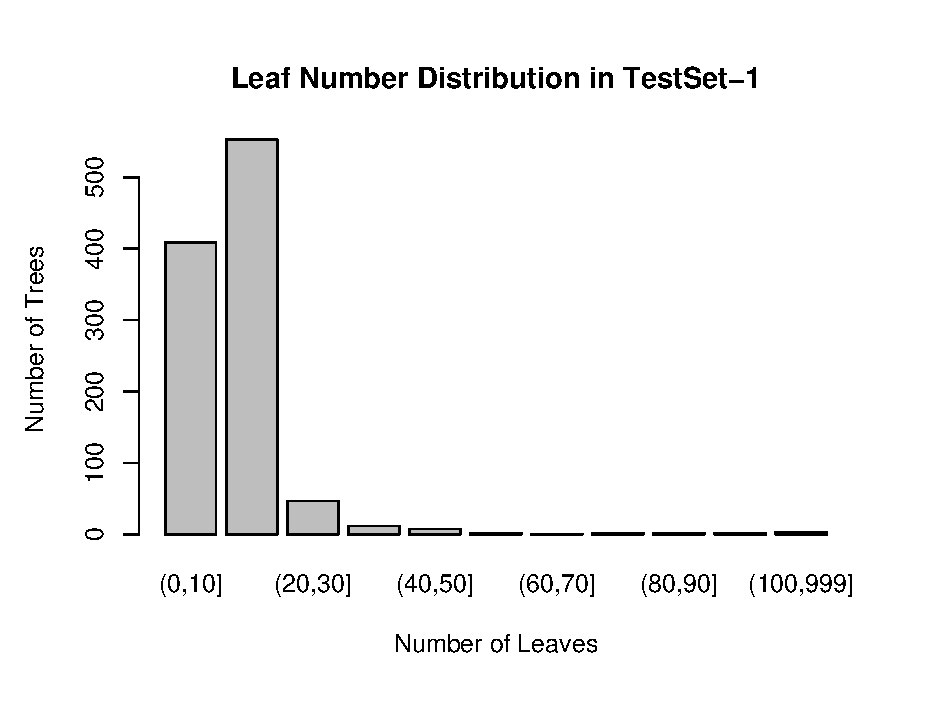
\includegraphics[width=0.49\textwidth]{leaf-ts1}
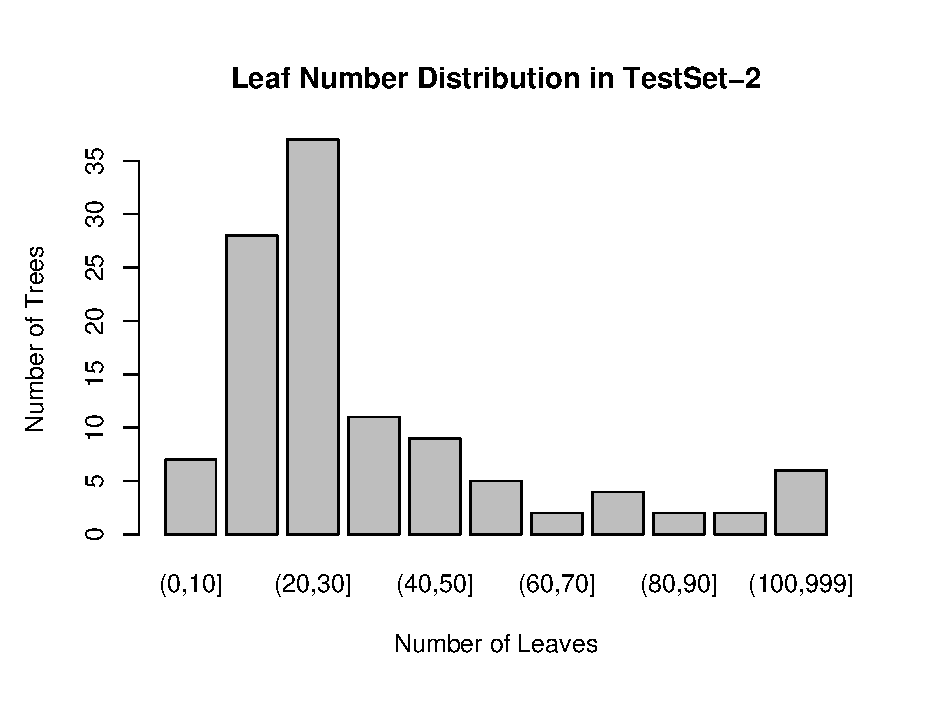
\includegraphics[width=0.49\textwidth]{leaf-ts2}
\end{center}
\caption{Distribution of number of leaves in {\sf TestSet1} and {\sf TestSet2}.}\label{fig:leaf-dist}
\end{figure}

\section{Measuring the Quality of Trees}

Two criteria were used to evaluate the quality of automatic trees. First, automatic trees were
compared with curated trees. Topological differences between them were measured by topological distance $dT$~\cite{robinson81},
which counts the number of branches that exist in one tree but not in the other~\cite{kuhner94}.
Topological distance $dT$ can be calculated given unrooted multifurcated trees. It equals to zero
if two trees are identical; it reaches its highest value $2n-6$, where $n$ is the number of
leaves in either tree, if two trees are completely different. Based on $dT$, the
distance between two methods $M_1$ and $M_2$ can be defined given $m$ multialignments:
\begin{equation}
d_M(M_1,M_2)=\frac{\sum_{i=1}^m{dT_i(M_1,M_2)}}{\sum_{i=1}^m{2n_i-6}}
\end{equation}
where $dT_i(M_1,M_2)$ is the topological distance between two trees reconstructed by the two methods based on
$i$-th multialignment, and $n_i$ is the number of sequences in the alignment.
Rescaled between 0 and 1, method distance $d_M$ is comparable between different test sets.
It, in fact, represents the percentage of branches that can only be
reconstructed by one method. In this thesis, differences between manual curation and automatic algorithms
are also measured by $d_M$.

Curated trees were processed from automatic methods. Their accuracy is inevitablely affected by
automatic methods in use. In addition, curation is a subjective process more or less, which might also make curated
trees deviate from the true history. To objectively measure the quality of automatic methods,
we also use percent duplications $p_D$ and average losses $p_L$ which are defined as:
\begin{eqnarray}
p_D(M) &=& \frac{\sum_{i=1}^m{D^*_i(M)}}{\sum_{i=1}^m{n_i-1}} \\
p_L(M) &=& \frac{\sum_{i=1}^m{L^*_i(M)}}{\sum_{i=1}^m{n_i-1}} 
\end{eqnarray}
where $D^*_i(M)$ is the number of duplications inferred from the tree reconstructed
by method $M$ from $i$-th alignment, and $L^*_i(M)$ is the number of losses. If we
accept the hypothesis that true phylogenies tend to contain fewer duplications and
losses, better methods must correspond to smaller $p_D$ and $p_L$. Although this
hypothesis might be violated in a few gene families, the overall trend should still
stand.

The two test sets only represent a small part of all Eukaryotic gene families.
To investigate the statistical reliability of our results, we designed a bootstrapping
procedure to calculate the standard deviation of each statistics, $p_D$, $p_L$ and $d_M$.
In {\sf TestSet2},
113 families were resampled with replacement for $B$ times, which forms $B$ sets of families
with each set containing 113 families.
Criterion $r_i$ was calculated from 113 resampled families for $i$-th round of resampling.
Mean value $\mu$ and SD (Standard Deviation) $\sigma$ were then estimated as:
\begin{eqnarray*}
\mu_r&=&\frac{\sum_i r_i}{B}\\
\sigma_r&=&\sqrt{\frac{\sum_i{r^2_i}-B\mu_r^2}{B-1}}
\end{eqnarray*}
A very small $\sigma_r$ means that a $r$ estimated from the original 113 families is similar to
the $r$ estimated from all animal families on the condition that these 113 families can represent all animal families.
In most cases, $\mu_r$ is almost identical to $r$ estimated from the original data, and
therefore $\mu_r$ will not be showed. Such calculation can also be applied to
{\sf TestSet1}. They are not showed as $\sigma_r$ on {\sf TestSet1} are similar to those
on {\sf TestSet2}.

\section{Accuracy of Tree Building Algorithms}

\begin{table}[!hb]
\begin{center}
\begin{tabular}{|l|cc|cc|cc|ccc|}
\hline
                 &\multicolumn{6}{|c|}{\sf TestSet2}             &\multicolumn{3}{|c|}{\sf TestSet1}\\
\hline
Type             &$d_M$ &$\sigma$&$p_D$ &$\sigma$&$p_L$ &$\sigma$&$d_M$  &$p_D$  &$p_L$  \\
\hline
{\tt CUR}        & 0.000 & 0.000 & 0.249 & 0.017 & 0.388 & 0.029 & 0.000 & 0.175 & 0.494 \\
\hline                                                                                   
{\tt NJ-NT-HKY4} & 0.225 & 0.017 & 0.313 & 0.017 & 0.786 & 0.042 & 0.133 & 0.204 & 0.630 \\
{\tt NJ-AA-WAG4} & 0.256 & 0.016 & 0.322 & 0.016 & 0.901 & 0.050 & 0.154 & 0.220 & 0.756 \\
{\tt NJ-NT-dN}   & 0.201 & 0.011 & 0.308 & 0.015 & 0.796 & 0.040 & 0.135 & 0.211 & 0.714 \\
{\tt NJ-NT-dS}   & 0.527 & 0.017 & 0.431 & 0.014 & 1.761 & 0.041 & 0.464 & 0.345 & 1.561 \\
{\tt NJ-AA-MM}   & 0.225 & 0.012 & 0.308 & 0.016 & 0.823 & 0.042 & 0.137 & 0.213 & 0.740 \\
{\tt NJ-AA-Kmr}  & 0.275 & 0.018 & 0.333 & 0.017 & 0.988 & 0.065 & 0.165 & 0.226 & 0.790 \\
{\tt ME-NT-HKY4} & 0.200 & 0.015 & 0.307 & 0.017 & 0.720 & 0.035 & 0.131 & 0.202 & 0.620 \\
{\tt ME-AA-WAG4} & 0.232 & 0.014 & 0.317 & 0.017 & 0.858 & 0.047 & 0.151 & 0.217 & 0.744 \\
\hline
{\tt PARS-NT}    & 0.203 & 0.013 & -     & -     & -     & -     & 0.151 & -     & -     \\
{\tt PARS-AA}    & 0.181 & 0.013 & 0.286 & 0.016 & 0.614 & 0.035 & 0.150 & 0.207 & 0.684 \\
\hline
{\tt ML-NT-HKY4} & 0.152 & 0.017 & 0.300 & 0.016 & 0.676 & 0.041 & 0.145 & 0.206 & 0.636 \\
{\tt ML-NT-HKY2} & 0.147 & 0.018 & 0.301 & 0.017 & 0.677 & 0.041 & 0.143 & 0.206 & 0.639 \\
{\tt ML-NT-HKY1} & 0.172 & 0.017 & 0.306 & 0.016 & 0.693 & 0.038 & 0.143 & 0.208 & 0.647 \\
{\tt ML-AA-WAG4} & 0.185 & 0.015 & 0.299 & 0.016 & 0.705 & 0.044 & 0.159 & 0.213 & 0.709 \\
\hline
{\tt NJ-NT-dM}   & 0.165 & 0.011 & 0.291 & 0.016 & 0.687 & 0.037 & 0.121 & 0.195 & 0.622 \\
{\tt MERGE}      & 0.092 & 0.015 & 0.259 & 0.016 & 0.457 & 0.033 & 0.111 & 0.178 & 0.503 \\
\hline
\end{tabular}
\caption[Performance of tree builders]{Performance of tree builders. In this table,
	$d$ is the topological distance between tree {\tt CUR} and each other tree.
	$p_D$ is percent duplication and $p_L$ the average loss. Standard deviation $\sigma$
	was calculated from 1000 times of resampling in {\sf TestSet2}. Both $p_D$ and $p_L$ are not available
	for {\tt PARS-NT} because it contains unresolved nodes.
	For $p_L$, the Pearson's correlation coefficient
	between the two sets is 0.970.}\label{tab:perform}
\end{center}
\end{table}

Table~\ref{tab:perform} shows the performance of tree-building algorithms and models.
Generally, the small SD reveals that each criterion is quite stable. Due to the
bias between {\sf TestSet2} and {\sf TestSet1}, percent duplication $p_D$ significantly
differs between the two sets. This, fortunately, does not affect the evaluation of
these algorithms. Between the two test sets, the Pearson's correlation coefficient of $p_D$ is 0.965,
and of $p_L$ is 0.970, which means that the results from the two sets highly agree with
each other.

Judged from the topological distance $d_M$ to the curated tree {\tt CUR},
tree {\tt MERGE} outperforms all the other methods on both test sets. On {\sf TestSet2},
this may be due to the fact that tree {\tt CUR} was curated from {\tt MERGE}, but
such an interpretation cannot account for the good performance on {\sf TestSet1}
where {\tt CUR} was curated from {\tt NJ-AA-MM} instead of {\tt MERGE}.
The similarity between {\tt CUR} and {\tt MERGE} on {\sf TestSet1} manifests that
human experts also favoured {\tt MERGE} even if they started from a less accurate tree.
Tree merge algorithm successfully captures the thinking of a biologist.

Judged from percent
duplication $p_D$ and average loss $p_L$, {\tt MERGE} is still the winner.
The number of duplications and losses inferred from this tree is significantly less.
The role of tree merge algorithm is also evident from {\tt NJ-NT-dM}. Merged
from {\tt NJ-NT-dN} and {\tt NJ-NT-dS}, two less accurate trees, this tree is even as accurate as those built by ML
with complex model.

So far as single-method trees are concerned, parsimony and ML methods show their power.
They are usually better than distance-based methods, except in one case where {\tt ME-NT-HKY4},
the tree built by FASTME, outperforms all the others on {\sf TestSet1}. Tree {\tt PARS-AA}
is the best on {\sf TestSet2}. But as it was merged from several parsimonious trees given by
{\bf protpars}, part of its high accuracy should attribute to the tree merge algorithm.
ML methods worked smoothly well on both sets, and on each criterion as well.
The role of applying $\Gamma$ distribution is revealed but very subtle.

As to distance-based methods, nucleotide model HKY is uniformly better than all amino acid models.
FASTME definitely outperforms standard neighbour-joining, which is in line with Desper and Gascuel~\cite{desper04}.
Notably, using complex evolutionary models at protein level does not guarantee higher accuracy at all.
This confirms the observation by Hollich {\it et al.}~\cite{hollich05}.

Figure~\ref{fig:phy-tree} shows the `phylogenies' of tree builders. `Signature' of different
tree building algorithms are evident: proteins-level methods and nucleotide-level methods
tend to be separated into two classes, while distance-based ones be grouped together.
Similar methods share similar properties. This also implies that tree merge can be more
helpful if trees with different properties are provided; otherwise common flaws
shared by a group of algorithms will never be overcome.

\begin{figure}[!hb]
\begin{center}
\includegraphics[width=\textwidth]{tree-0}\\
\includegraphics[width=\textwidth]{tree-1}
\caption[Relationships between tree builders]
{Relationships between tree builders. The top tree was built based on {\sf TestSet2}, and
the bottom on {\sf TestSet1}. Following the name of each leaf, the first number is percent duplication $p_D$
and the second average loss $p_L$. To build these two tree, topological distance $d$ between each pair of tree builders
was first calculated. Resultant distance matrix was then fed to NJTREE, which built the tree
by neighbour-joining. Bootstrapping procedure have been described above. 100 resampled
trees were finally combined together by {\bf CONSENSE} in {\bf PHYLIP} package. This
gave the supporting values on each branch.}\label{fig:phy-tree}
\end{center}
\end{figure}

\section{Discussion}
Properties of test data sets, such as divergence of sequences,
number of sequences in a tree, number of available sites in alignments,
and heterogeneity of site-specific rates, predetermine the performance
of each tree builder. This has been observed by many previous
studies~\cite{kuhner94,hall05,hollich05}. Consisting of real data from TreeFam,
our test sets represent a small number of families that date back to the last common
ancestor of Eukaryotes. Limited to the size and characteristics of data, we cannot
extensively study how each algorithm performs on various context. But as our benchmark
were carried on real data, the results may be of more practical importance.

Our work shows that tree merge algorithm is capable of
capturing the knowledge of biologists. It can greatly improve the accuracy of tree
reconstruction when the phylogeny of species is clear.
The success of tree merge also manifests that each class of single-model algorithm is able to build
part of correct branches that cannot be reconstructed by others; otherwise there must be
an algorithm that approaches the accuracy of tree {\tt MERGE}. As no single-method
algorithm can uniformly outperform all the others, it is always necessary to
combine trees with different algorithms if higher accuracy is desired.

On the other hand, tree merge only works well with Eukaryotic gene trees, where duplications
and losses can be inferred without the interference of LGT. On reconstruction of
species tree or bacterial gene trees, single-method algorithms are the only solution.
Our results suggest that each class of algorithms have their own strength. Although
parsimonious tree based on protein data and ML trees seem better in general,
distance-based method such as {\tt ME-NT-HKY4} can still outperform them at times.
Even when tree merge is not applicable, comprehensively investigating trees built
from different classes of algorithms is still always helpful.

\appendix
\chapter{Technical Issues}

\section{NJTREE Software}

NJTREE is the core engine of the whole TreeFam database. It realizes
almost all the algorithms described in this thesis, including
the cNJ algorithm (Section~\ref{sec:cnj}) for both rooted and unrooted constraining trees,
rooting and bootstrapping,
leaf reording algorithm (Section~\ref{sec:reorder}),
duplication/loss inference for multifurcated species trees (Chapter~\ref{chap:dli}),
and tree merge algorithm (Chapter~\ref{chap:merge}.
It also provides a lot of utilities facilitating the construction of TreeFam (Chapter~\ref{chap:treefam})
and the benchmark done in Chapter~\ref{chap:benchmark}.
In addition, NJTREE incorporates source codes from PHYML~\cite{guindon03},
which makes it capable of utilizing the power of ML methods.
To some extent, most parts of the thesis is describing the priciples behind this software.

NJTREE is efficient. It is much faster than any other neighbour-joining tree builders,
and can calculate max-likelihood distance in a speed not compared by other
similar softwares. Even NJTREE-revised PHYML codes runs 20\% faster than the original ones.
In addition, NJTREE comes with a nice graphical user interface (GUI), FLNJTREE, which is built upon
FLTK (fast light-weighted toolkit), a cross-platform widget library. FLNJTREE
can be compiled in both UNIX (including LINUX) and Windows. In theory, it should also work in Mac OSX, though this
has not been tested. Figure~\ref{fig:flnjtree} shows a snapshot of FLNJTREE.

\begin{figure}[!hb]
\includegraphics[width=\textwidth]{flnjtree.png}
\caption{Screenshot of FLNJTREE software.}\label{fig:flnjtree}
\end{figure}

\section{MySQL Structures}
TreeFam database is supported on \href{http://www.mysql.com/}{MySQL}, probably
the most popular open source database in the world. Except the original
PhIGs alignment, all the other data are stored in the relational database.
The structures of TreeFam MySQL schema are very intuitive.
Most the tables can be classified into three groups: tables for describing
gene attributes, tables for recording family information, and tables connecting
the two parts. Table~\ref{tab:mysql-table} gives a brief list of key tables
in TreeFam database, and Figure~\ref{fig:schemata} shows the relations between them.
Note that in TreeFam MySQL tables, gene identifiers and family accessions are
directly used as index. This is clearer than using integer ID, but is ineffiecient from
a pure technical angle~\footnote{\href{http://www.informit.com/articles/article.asp?p=377652\&seqNum=1}
{http://www.informit.com/articles/article.asp?p=377652\&seqNum=1}}. As efficiency seems not a serious problem at present,
we can live with this for the moment. TreeFam MySQL database is open to public at
{\bf db.treefam.org:3308}. The read-only account is {\bf anonymous} with empty password.

\begin{figure}[!hb]
\includegraphics[width=\textwidth]{schemata.png}
\caption[Schema of TreeFam database]{Schema of TreeFam database. This figure is generated by
\href{http://www.fabforce.net/dbdesigner4/}{DBDesigner4}.}\label{fig:schemata}
\end{figure}

\begin{table}[!hb]
\begin{center}
\begin{tabular}{|l|l|}
\hline
Table & Description \\
\hline
genes & sequence ID, gene name, transcript name, symbol, description and so on \\
species & tax ID, taxonomy name, {\it abbr.} name, and common name of species \\
map & genomic locations of transcripts; in UCSC format \\
pfam & Pfam predictions for each sequence \\
aa\_seq & amino acid sequences \\
nt\_seq & nucleotide sequences \\
familyA & accessions, symbols and names of TreeFam-A families \\
familyB & basic information on TreeFam-B families \\
famB2A & relation between curated TreeFam-A and original TreeFam-B families \\
phigs & PhIGs accessions of TreeFam-B families \\
trees & phylogenetic trees in NHX format \\
misc\_feat & symbols and names of B families; curators of A families \\
misc\_key & descriptions of `key' used in `misc\_feat' table \\
aa\_seed\_align & amino acids multialignment for TreeFam-A seeds in CIGAR format \\
aa\_full\_align & full multialignment for both A and B families in CIGAR format \\
hmmer & HMMer scores of matched sequences \\
\hline
\end{tabular}
\end{center}
\caption[Description of key TreeFam MySQL tables]{Description of key TreeFam MySQL tables. Trivial or obsolete ones
are not included.}\label{tab:mysql-table}
\end{table}

\section{Perl API}
It is recommended to connect TreeFam MySQL with perl API, which
provides convenient interface for the retrieval of various TreeFam data. TreeFam API
also implements a light-weighted parser for NHX format, a versatile tree plotter and
a simple alignment plotter. Full documentation is available at
\href{http://www.treefam.org/api/}{http://www.treefam.org/api/}.
%We only show some practical examples here as an introduction.

\chapter{Publications}

{
\setlength{\parindent}{0pt}
\setlength{\parskip}{1.2ex plus 0.5ex minus 0.2ex}

% \bibitem[Li {\em et~al.}, 2006]{myli06}
\underline{Li,H.}, Coghlan,A., Ruan,J., Coin,L.J., H{\'e}rich{\'e},J.K., Osmotherly,L.,
  Li,R., Liu,T., Zhang,Z., Bolund,L., Wong,G.K., Zheng,W., Dehal,P., Wang,J.
  and Durbin,R. (2006{\em{}}) Treefam: a curated database of phylogenetic trees
  of animal gene families.
\newblock {\em Nucleic Acids Res, } {\bf 34} (Database issue), 572--580. (first author)

% \bibitem[Yu {\em et~al.}, 2005]{myyu05}
Yu,J., Wang,J., Lin,W., Li,S., \underline{Li,H.}, Zhou,J., Ni,P., Dong,W., Hu,S., Zeng,C.,
  Zhang,J., Zhang,Y., Li,R., Xu,Z., Li,S., Li,X., Zheng,H., Cong,L., Lin,L.,
  Yin,J., Geng,J., Li,G., Shi,J., Liu,J., Lv,H., Li,J., Wang,J., Deng,Y.,
  Ran,L., Shi,X., Wang,X., Wu,Q., Li,C., Ren,X., Wang,J., Wang,X., Li,D.,
  Liu,D., Zhang,X., Ji,Z., Zhao,W., Sun,Y., Zhang,Z., Bao,J., Han,Y., Dong,L.,
  Ji,J., Chen,P., Wu,S., Liu,J., Xiao,Y., Bu,D., Tan,J., Yang,L., Ye,C.,
  Zhang,J., Xu,J., Zhou,Y., Yu,Y., Zhang,B., Zhuang,S., Wei,H., Liu,B., Lei,M.,
  Yu,H., Li,Y., Xu,H., Wei,S., He,X., Fang,L., Zhang,Z., Zhang,Y., Huang,X.,
  Su,Z., Tong,W., Li,J., Tong,Z., Li,S., Ye,J., Wang,L., Fang,L., Lei,T.,
  Chen,C., Chen,H., Xu,Z., Li,H., Huang,H., Zhang,F., Xu,H., Li,N., Zhao,C.,
  Li,S., Dong,L., Huang,Y., Li,L., Xi,Y., Qi,Q., Li,W., Zhang,B., Hu,W.,
  Zhang,Y., Tian,X., Jiao,Y., Liang,X., Jin,J., Gao,L., Zheng,W., Hao,B.,
  Liu,S., Wang,W., Yuan,L., Cao,M., McDermott,J., Samudrala,R., Wang,J.,
  Wong,G.  and Yang,H. (2005{\em{}}) {The Genomes of Oryza sativa: a history of
  duplications}.
\newblock {\em PLoS Biol, } {\bf 3} (2). (co-first author)

% \bibitem[Li {\em et~al.}, 2005]{myli05}
\underline{Li,H.}, Liu,J., Xu,Z., Jin,J., Fang,L., Gao,L., Li,Y., Xing,Z., Gao,S., Liu,T.,
  Li,H., Li,Y., Fang,L., Xie,H., Zheng,W.  and Hao,B. (2005{\em{}}) {Test data
  sets and evaluation of gene prediction programs on the rice genome}.
\newblock {\em J Comput Sci \& Technol, } {\bf 20} (4), 446--453. (first author)

% \bibitem[Wong {\em et~al.}, 2004]{mywong04}
Wong,G., Liu,B., Wang,J., Zhang,Y., Yang,X., Zhang,Z., Meng,Q., Zhou,J., Li,D.,
  Zhang,J., Ni,P., Li,S., Ran,L., \underline{Li,H.}, Zhang,J., Li,R., Li,S., Zheng,H.,
  Lin,W., Li,G., Wang,X., Zhao,W., Li,J., Ye,C., Dai,M., Ruan,J., Zhou,Y.,
  Li,Y., He,X., Zhang,Y., Wang,J., Huang,X., Tong,W., Chen,J., Ye,J., Chen,C.,
  Wei,N., Li,G., Dong,L., Lan,F., Sun,Y., Zhang,Z., Yang,Z., Yu,Y., Huang,Y.,
  He,D., Xi,Y., Wei,D., Qi,Q., Li,W., Shi,J., Wang,M., Xie,F., Wang,J.,
  Zhang,X., Wang,P., Zhao,Y., Li,N., Yang,N., Dong,W., Hu,S., Zeng,C.,
  Zheng,W., Hao,B., Hillier,L., Yang,S., Warren,W., Wilson,R.,
  Brandstr{\"o}m,M., Ellegren,H., Crooijmans,R., van~der Poel,J., Bovenhuis,H.,
  Groenen,M., Ovcharenko,I., Gordon,L., Stubbs,L., Lucas,S., Glavina,T.,
  Aerts,A., Kaiser,P., Rothwell,L., Young,J., Rogers,S., Walker,B., van
  Hateren,A., Kaufman,J., Bumstead,N., Lamont,S., Zhou,H., Hocking,P.,
  Morrice,D., de~Koning,D., Law,A., Bartley,N., Burt,D., Hunt,H., Cheng,H.,
  Gunnarsson,U., Wahlberg,P., Andersson,L., Kindlund,E., Tammi,M.,
  Andersson,B., Webber,C., Ponting,C., Overton,I., Boardman,P., Tang,H.,
  Hubbard,S., Wilson,S., Yu,J., Wang,J.  and Yang,H. (2004{\em{}}) {A genetic
  variation map for chicken with 2.8 million single-nucleotide polymorphisms}.
\newblock {\em Nature, } {\bf 432} (7018), 717--722.

% \bibitem[Xia {\em et~al.}, 2004]{myxia04}
Xia,Q., Zhou,Z., Lu,C., Cheng,D., Dai,F., Li,B., Zhao,P., Zha,X., Cheng,T.,
  Chai,C., Pan,G., Xu,J., Liu,C., Lin,Y., Qian,J., Hou,Y., Wu,Z., Li,G.,
  Pan,M., Li,C., Shen,Y., Lan,X., Yuan,L., Li,T., Xu,H., Yang,G., Wan,Y.,
  Zhu,Y., Yu,M., Shen,W., Wu,D., Xiang,Z., Yu,J., Wang,J., Li,R., Shi,J.,
  \underline{Li,H.}, Li,G., Su,J., Wang,X., Li,G., Zhang,Z., Wu,Q., Li,J., Zhang,Q.,
  Wei,N., Xu,J., Sun,H., Dong,L., Liu,D., Zhao,S., Zhao,X., Meng,Q., Lan,F.,
  Huang,X., Li,Y., Fang,L., Li,C., Li,D., Sun,Y., Zhang,Z., Yang,Z., Huang,Y.,
  Xi,Y., Qi,Q., He,D., Huang,H., Zhang,X., Wang,Z., Li,W., Cao,Y., Yu,Y.,
  Yu,H., Li,J., Ye,J., Chen,H., Zhou,Y., Liu,B., Wang,J., Ye,J., Ji,H., Li,S.,
  Ni,P., Zhang,J., Zhang,Y., Zheng,H., Mao,B., Wang,W., Ye,C., Li,S., Wang,J.,
  Wong,G.  and Yang,H. (2004{\em{}}) {A draft sequence for the genome of the
  domesticated silkworm (Bombyx mori)}.
\newblock {\em Science, } {\bf 306} (5703), 1937--1940.

% \bibitem[Wang {\em et~al.}, 2004]{mywang04}
Wang,J., Zhang,J., Zheng,H., Li,J., Liu,D., \underline{Li,H.}, Samudrala,R., Yu,J.  and
  Wong,G. (2004{\em{}}) {Mouse transcriptome: neutral evolution of 'non-coding'
  complementary DNAs}.
\newblock {\em Nature, } {\bf 431} (7010), 1--1.

% \bibitem[Li {\em et~al.}, 2004]{myli04}
Li,C., Ni,P., Francki,M., Hunter,A., Zhang,Y., Schibeci,D., \underline{Li,H.}, Tarr,A.,
  Wang,J., Cakir,M., Yu,J., Bellgard,M., Lance,R.  and Appels,R. (2004{\em{}})
  {Genes controlling seed dormancy and pre-harvest sprouting in a
  rice-wheat-barley comparison}.
\newblock {\em Funct Integr Genomics, } {\bf 4} (2), 84--93.

}


\refstepcounter{chapter}
\addcontentsline{toc}{chapter}{Bibliography}
\bibliography{ref}

\refstepcounter{chapter}
\addcontentsline{toc}{chapter}{Index}
\printindex

\end{document}
